% double-spaced format
\documentclass[12pt,twoside]{article}
\usepackage{setspace}

% ACM format
%\documentclass{sig-alternate}
%\newcommand{\setstretch}[1]{}
%\newenvironment{singlespace}{}

\usepackage{smaller}
\usepackage{algorithm}
\usepackage{algorithmic}
\usepackage{lgrind}
\usepackage{simplemargins}
\usepackage{times}
\usepackage{epsfig}

%\title{Optimizing Stream Programs \\ Using a Linear State Space Representation}
%\title{A Linear State Space Representation \\ for Optimizing Stream Programs}
\title{\vspace*{-0.5in}\smaller {\bf Optimizing Stream Programs Using Linear State Space Analysis}}
 \author{~ \vspace{-24pt} \\ Sitij Agrawal, William Thies, and Saman Amarasinghe \\[0.2Ex]
   MIT Computer Science and Artificial Intelligence Laboratory}
%   \normalsize\tt{\{sitij, thies, saman\}@csail.mit.edu}}

% don't include the date
\date{}

\setallmargins{0.8in}

% this is the line spacing
\setstretch{1.78}

% \sloppy lets Latex be a little less anal about interword spacing.  It is
% one way to eliminate those annoying Overfull hbox warnings.
% Another way is to surround each offending paragraph with
% \begin{sloppypar} ... \end{sloppypar}

%\sloppy

% See page 90 of the Latex book for info about vertical spacing probs.

\begin{document}

  \newcommand{\subsubsubsection}[1]{\medskip\noindent{\bf #1}\\\smallskip}
  \newcommand{\mt}[1]{\mbox{\it #1}}
  \newcommand{\todo}[1]{\framebox{#1}}
  \newcommand{\vc}[1]{\vec{#1}}
  
  % shrink the itemized lists
  \newlength{\itemshrink}
  \setlength{\itemshrink}{-12pt}
  %\setlength{\itemshrink}{0pt}

  % shrink spacing of section titles
  \newcommand{\mysection}[1]{\vspace{-23pt} \section{#1} \vspace{-12pt}}
  \newcommand{\mysubsection}[1]{\vspace{-17pt} \subsection{#1} \vspace{-12pt}}
  \newcommand{\mysubsubsection}[1]{\vspace{-17pt} \subsubsection{#1} \vspace{-12pt}}
%  \newcommand{\mysection}[1]{\section{#1}}
%  \newcommand{\mysubsection}[1]{\subsection{#1}}
%  \newcommand{\mysubsubsection}[1]{\subsubsection{#1}}

  % proper spacing of equations
%  \newcommand{\starteqnstar}[0]{\begin{eqnarray*}}
%  \newcommand{\doneeqnstar}[0]{\end{eqnarray*}}
%  \newcommand{\starteqn}[0]{\begin{eqnarray}}
%  \newcommand{\doneeqn}[0]{\end{eqnarray}}

   \newlength{\topeqn}
   \setlength{\topeqn}{-24pt}
   \newlength{\boteqn}
   \setlength{\boteqn}{-24pt}
   \newcommand{\starteqnstar}[0]{\begin{singlespace}\vspace{\topeqn}\begin{eqnarray*}}
   \newcommand{\doneeqnstar}[0]{\end{eqnarray*}\vspace{\boteqn}\end{singlespace}}
   \newcommand{\starteqn}[0]{\begin{singlespace}\begin{eqnarray}\vspace{\topeqn}}
   \newcommand{\doneeqn}[0]{\end{eqnarray}\vspace{\boteqn}\end{singlespace}}

  %\toappear{\centerline{\Large\bf MIT LCS Technical Memo,}
  %          \centerline{\Large\bf MIT-LCS-TM-6XX,}
  %          \centerline{\Large\bf November, 2001.}}
  
  \begin{singlespace}
    \maketitle
    \vspace{-20pt}
    \begin{abstract}
      As DSP programming is becoming more complex, there is an increasing
need for high-level abstractions that can be efficiently compiled.
Toward this end, we present a set of aggressive optimizations that
target linear sections of a stream program.  Our input language is
StreamIt, which represents programs as a hierarchical graph of
autonomous filters.  A filter is linear if each of its outputs can be
represented as an affine combination of its inputs.  Linear filters
are common in DSP applications; examples include FIR filters,
expanders, compressors, FFTs and DCTs.

We present a linear extraction analysis that automatically detects
linear filters based on the C-like code in their {\tt work} function.
Once linear filters are identified, we show how neighboring nodes can
be collapsed into a single linear representation, thereby eliminating
many redundant computations.  Also, we describe a method for
automatically translating linear nodes into the frequency domain,
thereby yielding algorithmic savings for convolutional filters.

We have completed a fully-automatic implementation of the above
techniques as part of the StreamIt compiler, and we demonstrate
performance improvements that average 400\% over our benchmark
applications.




    \end{abstract}
  \end{singlespace}
  
%  \advance\topmargin by -0.35in      % Correct for LaTeX gratuitousness

  \section{Introduction}

Applications that are structured around some notion of a ``stream''
are becoming increasingly important and widespread.  There is evidence
that streaming media applications are already consuming most of the
cycles on consumer machines \cite{Rix98}, and their use is continuing
to grow.  In the embedded domain, applications for hand-held
computers, cell phones, and DSP's are centered around a stream of
voice or video data.  The stream abstraction is also fundamental to
high-performance applications such as intelligent software routers,
cell phone base stations, and HDTV editing consoles.

Despite the prevalence of these applications, there is surprisingly
little language and compiler support for practical, large-scale stream
programming.  Of course, the notion of a stream as a programming
abstraction has been around for decades \cite{SICP}, and a number of
special-purpose stream languages have been designed (see
\cite{survey97} for a review).  Many of these languages and
representations are elegant and theoretically sound, but they often
lack features and are too inflexible to support straightforward
development of modern stream applications, or their implementations
are too inefficient to use in practice.  Consequently, most
programmers turn to general-purpose languages such as C or C++ to
implement stream programs.

There are two reasons that general-purpose languages are inadequate for
stream programming.  Firstly, they are a mismatch for the application
domain.  That is, they do not provide a natural or intuitive
representation of streams, thereby having a negative effect on
readability, robustness, and programmer productivity.  Moreover, because
the widespread parallelism and regular communication patterns of data
streams are left implicit in general-purpose languages, compilers are
not stream-conscious and do not perform stream-specific optimizations.
As a result, performance-critical loops are often hand-coded in a
low-level assembly language and must be re-implemented for each target
architecture.  This practice is labor-intensive, error-prone, and very
costly.

Secondly, general-purpose languages are a mismatch for the emerging
class of grid-based architectures \cite{smartmemories,rawshort,trips} that
are especially well-suited for stream processing.  Perhaps the primary
appeal of C is that it provides a ``common machine language'' for
von-Neumann architectures.  That is, it abstracts away the
idiosyncratic differences between machines, but encapsulates their
common properties: a single program counter, arithmetic operations,
and a monolithic memory.  However, for grid-based architectures, the
von-Neumann model no longer holds, as there are multiple instruction
streams and distributed memory banks.  Thus, C no longer serves as a
common machine language--in fact, it provides the wrong abstraction
for the underlying hardware, and architecture-specific directives are
often needed to obtain reasonable performance.  Again, this greatly
complicates the job of the programmer and hampers portability.

StreamIt is a language and compiler specifically designed for modern
stream programming.  The StreamIt language has two goals: first, to
provide high-level stream abstractions that improve programmer
productivity and program robustness within the streaming domain, and
second, to serve as a common machine language for grid-based
processors.  At the same time, the StreamIt compiler aims to perform
stream-specific optimizations to achieve the performance of an expert
programmer.

This paper motivates, describes, and justifies the high-level language
features of StreamIt, version 1.0.  The major limitation of StreamIt
1.0 is that all flow rates in the streams must be static; applications
such as compression that have dynamically varying flow rates will be
the subject of future work.  A large set of applications can be
implemented with static rates, and while dynamic rates will require a
different runtime model, it will still be essential to fully analyse
and optimize static sub-sections in order to obtain high performance.

The paper is organized as follows. In Section {\ref{sec:domain}}, we
characterize the domain of streaming programs that motivates the
design of StreamIt, and in Section~\ref{sec:overview} we describe the
language features in detail.  We present an in-depth example of a
software radio in Section~\ref{sec:example}, preliminary results in
Section~\ref{sec:results}, related work in Section~\ref{sec:related},
and conclusions in Section~\ref{sec:conc}.


  \begin{figure}[t]
{\scriptsize
\begin{verbatim}
   float->float filter MovingAverage(int N) {
     float[N] weights;  // a filter field

     // init function initializes the weights
     init {
       for (int i=0; i<N; i++)
         weights[i] = 1/N;
     }

     // work function declares push, pop, peek rates
     work push 1 pop 1 peek N {
       float result = 0;  // a local variable
       for (int i=0; i<N; i++) {
         result += weights[i] * peek(i);
       }
       push(result);
       pop();
     }
   } 
\end{verbatim}
\vspace{-12pt}
\caption{Example of a StreamIt filter.\protect\label{fig:filter-example}}}
\vspace{-6pt}
\end{figure}

\mysubsection{The StreamIt Language}
\label{sec:background}

StreamIt~\cite{streamitcc} is an architecture-independent language for
signal processing applications.  StreamIt aims to expose the abundant
parallelism and regular communication patterns in stream programs for
the benefit of the compiler.  The optimizations described in this
paper would be infeasible in a general-purpose language such as C.  As
detailed elsewhere~\cite{streamitcc}, C obscures the high-level
structure of a streaming application due to possible aliasing between
autonomous filters, complex modulo expressions on circular buffers,
and muddling of atomic execution steps with global control flow.
%There is not enough information in C code to automatically perform the
%high-level transformations that experts use to achieve competitive
%performance.  
In addition, StreamIt offers improved programmer productivity over C
due to its parameterizable and composable stream constructs.

The basic programmable unit in StreamIt is a filter; for example, see
the {\tt MovingAverage} filter in Figure~\ref{fig:filter-example}.  A
filter contains a work function which executes atomically, popping a
fixed number of items from the filter's input tape and pushing a fixed
number of items to the filter's output tape.  A filter can also
``peek'' at a given index on its input tape without consuming the
item; this makes it simple to write sliding-window applications such
as the {\tt MovingAverage}.  The push, pop, and peek rates are
declared on the same line as the work function, thereby enabling the
compiler to construct a static schedule of filter
firings~\cite{lee87static}.

Each filter has a distinct address space.  A filter can store two
types of variables: a {\it field} and a {\it local}.  Fields are
declared in the scope of the filter and are preserved across
executions, while locals are declared inside the work function and are
only live within a single execution.  There is also an init function,
run once at the beginning of the program, that can be used to
initialize fields.

StreamIt provides three hierarchical structures for composing filters
into larger stream graphs (see Figure~\ref{fig:structures}).  The {\it
pipeline} construct composes streams in sequence, with the output of
one connected to the input of the next.  The {\it splitjoin} construct
distributes data to a set of parallel streams, which are then joined
together in a roundrobin fashion.  The {\it feedback loop} provides a
mechanism for introducing cycles in the graph.  An example of a
pipeline appears in Figure~\ref{fig:iir-pipeline}.  It contains a
single IIR (Infinite Impulse Response) filter, which could be
implemented as shown at the top of Figure~\ref{fig:opt-seq}.

%%         A filter can store two types of variables - \textit{field} and
%% \textit{local}. Field variables are declared outside of the
%% specific functions (work, prework, init), and can be accessed from
%% anywhere within the filter. Local variables are declared within a
%% specific function, and only have scope within that function. For
%% example, a variable declared within the init function is local,
%% and could not be accessed within the work function. Therefore, the
%% init function is used to initialize field variables.

\mysubsection{State Space Example}
\begin{figure}[t!]
\vspace{-14pt}
\begin{singlespace}
\hfill
\begin{minipage}{2.2in}
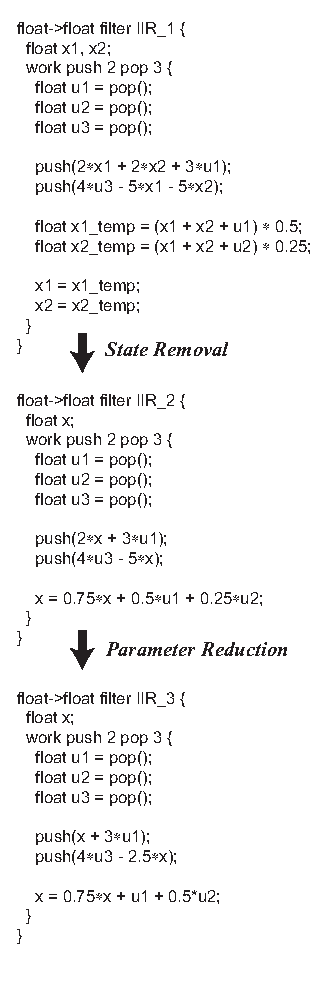
\epsfig{file=statespace-example.eps, width=2.05in}
\end{minipage}
~~~~
\raisebox{10pt}{
\begin{minipage}{3.5in}
\vspace{10pt}
{\small
Number of multiplications: 8 \\
Number of additions: 8 \\
State space representation:
}
\begin{eqnarray*}
\small
\vec{\mathbf{y}} & = & \left [ \begin{array} {cc} 2 & 2 \\ -5 & -5
\end{array} \right ] \vec{\mathbf{x}} + \left [ \begin{array} {ccc} 3 & 0 & 0 \\ 0 & 0 & 4 \end{array} \right
 ] \vec{\mathbf{u}} \\
\vec{\dot{\mathbf{x}}} & = & \left [ \begin{array} {cc} 0.5 & 0.5 \\ 0.25
& 0.25 \end{array} \right ] \vec{\mathbf{x}} + \left [ \begin{array} {ccc} 0.5 & 0 & 0 \\
0 & 0.25 & 0 \end{array} \right ] \vec{\mathbf{u}}
\end{eqnarray*}
\vspace{-3pt} ~ \\
\hrule
\vspace{26pt} ~ \\
{\small
Number of multiplications: 7 \\
Number of additions: 4 \\
State space representation:}
\begin{eqnarray*}
\small
\vec{\mathbf{y}} & = & \left [ \begin{array} {cc} 2 \\ -5
\end{array} \right ] \vec{\mathbf{x}} + \left [ \begin{array} {ccc} 3 & 0 & 0 \\ 0 & 0 & 4 \end{array} \right
 ] \vec{\mathbf{u}} \\
\vec{\dot{\mathbf{x}}} & = & \left [ \begin{array} {cc} 0.75
\end{array} \right ] \vec{\mathbf{x}} + \left [ \begin{array} {ccc} 0.5 & 0.25 & 0 \end{array} \right ] \vec{\mathbf{u}}
\end{eqnarray*}
\hrule
\vspace{12pt} ~ \\
{\small
Number of multiplications: 5 \\
Number of additions: 4 \\
State space representation:}
\begin{eqnarray*}
\small
\vec{\mathbf{y}} & = & \left [ \begin{array} {cc} 1 \\ -2.5
\end{array} \right ] \vec{\mathbf{x}} + \left [ \begin{array} {ccc} 3 & 0 & 0 \\ 0 & 0 & 4 \end{array} \right
 ] \vec{\mathbf{u}} \\
\vec{\dot{\mathbf{x}}} & = & \left [ \begin{array} {cc} 0.75
\end{array} \right ] \vec{\mathbf{x}} + \left [ \begin{array} {ccc} 1 & 0.5 & 0 \end{array} \right ] \vec{\mathbf{u}}
\end{eqnarray*}
\end{minipage}}
\end{singlespace}
\begin{center}
\vspace{-24pt}
\caption{Example optimization of an IIR filter using linear state
space analysis.  The top segment shows the original code.  The middle
segment depicts the action of state removal, in which the quantity
$x_1 + x_2$ is replaced by a single variable $x$.  The bottom segment
illustrates parameter reduction, in which the coefficients are
refactored to eliminate two multiplications (two coefficients
assume a value of 1).\protect\label{fig:opt-seq}}
\end{center}
\vspace{-18pt}
\hrule
\vspace{-12pt}
\end{figure}


As described previously, a linear state space model describes a stream
in which both the outputs and the state values are updated as a linear
combination of the inputs and the previous states.  We use the
following notation to describe such systems:
\starteqnstar 
\vec{\mathbf{y}}
& = & \mathbf{C}\vec{\mathbf{x}} + \mathbf{D}\vec{\mathbf{u}} \\
\vec{\dot{\mathbf{x}}} & = & \mathbf{A}\vec{\mathbf{x}} +
\mathbf{B}\vec{\mathbf{u}} \
\doneeqnstar
\noindent In these equations, the state vector is denoted by
$\vec{\mathbf{x}}$, the inputs by $\vec{\mathbf{u}}$, and the outputs
by $\vec{\mathbf{y}}$. $\vec{\dot{\mathbf{x}}}$ represents the new
state vector, i.e. the state vector after it is updated. The first
equation is for the outputs, while the second equation is for the
state updates.  $\mathbf{A}$, $\mathbf{B}$, $\mathbf{C}$, and
$\mathbf{D}$ are matrices whose dimensions depend on the number of
states, inputs, and outputs.  

Figure~\ref{fig:opt-seq} illustrates an optimization sequence for an
IIR filter.  Three versions of the filter are shown: original,
following state removal, and following parameter reduction.  In each
case, the state space representation for the filter is shown on the
right, along with the number of multiplications and additions needed
per execution of the work function.

The state removal optimization identifies that the states $x_1$ and
$x_2$ are always used as part of the expression $x_1 + x_2$.  Thus,
one of the states can be eliminated in favor of a single variable,
$x$, that tracks the value of the sum.  While relatively simple in
this example, such a transformation can be quite subtle when applied
to a large representation (e.g., the result of combining many filters
together.)  State removal can reduce storage requirements as well as
eliminate arithmetic operations (in this example, 1 multiplication and
4 additions).  As described in Section~\ref{sec:state-removal}, state
removal is formulated as a general sequence of matrix operations.

The parameter reduction optimization refactors the coefficients that
operate on the state variables in order to reduce the number of
operations needed.  Following the transformation, $x$ assumes a value
that is twice as large as the original (at any given point of
execution).  However, this change does not affect the output of the
filter, as the coefficients in $\mathbf{A}$ are compensated
accordingly.  The transformation enables two coefficients in $\mathbf{D}$
to change to a value of 1, thereby eliminating two multiplication
operations.  As described in Section~\ref{sec:parameter-reduction},
this transformation is also formulated as a general series of matrix
operations.

%%     StreamIt is a programming language specifically tailored to DSP
%% streaming applications. The user creates a graph composed of four
%% types of StreamIt constructs: \textit{filters},
%% \textit{pipelines}, \textit{splitjoins}, and \textit{feedback
%% loops}. Filters encapsulate the computation done within an
%% application - they represent the blocks mentioned in the previous
%% section. Each filter operates on a one-dimensional `tape' of
%% values (of any type, including structures and arrays).  The other
%% three constructs dictate the type of connections possible between
%% filters. Every construct explicitly states its input type and
%% output type, and can be passed parameters as would be to a
%% procedure.

%%     StreamIt uses a buffer between every pair of filters to
%% hold values. When the input buffer of a construct (equivalent to
%% the output buffer of the previous construct) is appropriately
%% filled, the construct can execute. Execution involves three steps:
%% reading and removing items from the input buffer (consumption);
%% performing computations; putting items in the output buffer
%% (production). We will not consider the intricacies of managing
%% these buffers, and instead refer to the more abstract notion of a
%% tape.

%%     A filter has pre-defined \textit{peek}, \textit{pop}, and
%% \textit{push} rates (StreamIt code examples are given below).
%% During each execution, the filter accesses a maximum of peek
%% values from its input tape, consumes exactly pop input values from
%% its input tape, and produces exactly push values onto its output
%% tape. Since the removal of an input value is technically an access
%% of that input, the peek rate of a filter must be greater than or
%% equal to the pop rate of that filter. The push or pop rate can be
%% zero - the former corresponds to a filter that consumes items but
%% does not produce them (typically the last filter in a sequence)
%% and the latter corresponds to a filter that produces items but
%% does not consume them (typically the first filter in a sequence).
%% All the accesses, outputs, and removals, as well as all the
%% computation is done inside the main body of the filter, known as
%% the work function.

%% \begin{figure}[bthp]
%%   \centering
%%   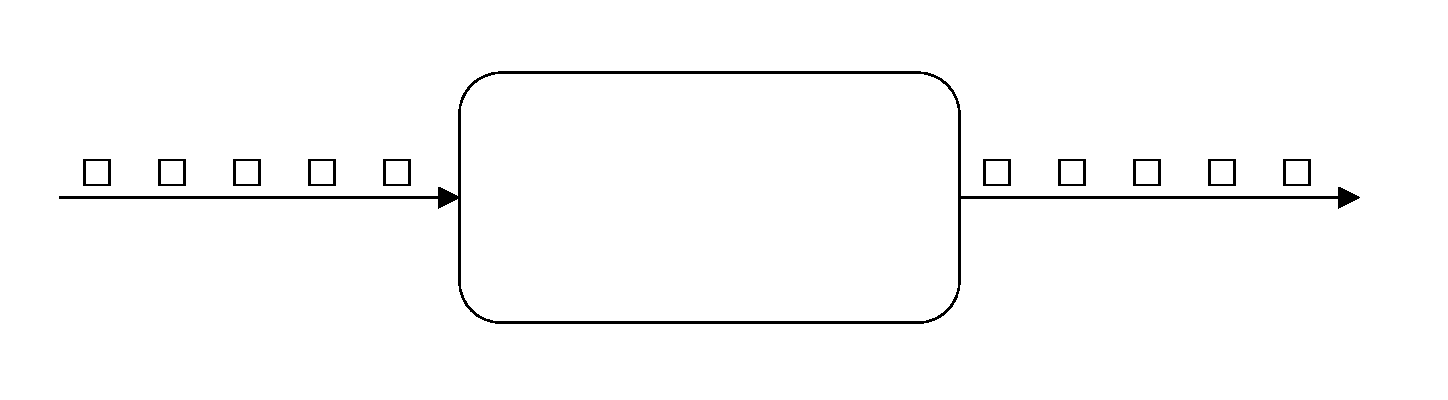
\includegraphics[width=3.0in]{figures/filter.eps}
%%   \caption{StreamIt filter}
%%   \label{fig:filter}
%% \end{figure}

%%     StreamIt also supports a \textit{prework} function, which has its own push,
%% pop, and peek rates.  The prework function executes in place of
%% the work function for the first computation sequence, and is never
%% run again. Additionally, there is an \textit{init} function which
%% is run only once upon creation of the filter, and is usually used
%% to initialize variables.  The init and prework functions are both
%% optional.

%%         A filter can store two types of variables - \textit{field} and
%% \textit{local}. Field variables are declared outside of the
%% specific functions (work, prework, init), and can be accessed from
%% anywhere within the filter. Local variables are declared within a
%% specific function, and only have scope within that function. For
%% example, a variable declared within the init function is local,
%% and could not be accessed within the work function. Therefore, the
%% init function is used to initialize field variables.

%% Code examples of StreamIt filters are shown below.

%% \begin{scriptsize}
%% \begin{singlespace}
%% \begin{verbatim}
%% // This filter adds the parameter scalar to each input.
%% // It does not have an init or prework function
%% float -> float filter scalarAdd(float scalar) {
%%   work push 1 pop 1 peek 1 {
%%     push(scalar + pop());
%%   }
%% }
%% \end{verbatim}
%% \end{singlespace}
%% \end{scriptsize}

%% \begin{scriptsize}
%% \begin{singlespace}
%% \begin{verbatim}
%% // This filter outputs a running average of every three consecutive inputs.
%% // The first time it runs, it ouputs the average of the first two inputs without removing anything from the tape.
%% // It does not have an init function.
%% float -> float filter threeWayAverage() {
%%   prework push 1 pop 0 peek 2 {
%%     float temp;  // example of a local variable
%%     temp = (peek(0)+peek(1))/2;
%%     push(temp);
%%   }
%%   work push 1 pop 1 peek 3 {
%%     float temp;  // example of a local variable
%%     temp = (peek(0) + peek(1) + peek(2))/3
%%     push(temp);
%%     pop()
%%   }
%% }
%% \end{verbatim}
%% \end{singlespace}
%% \end{scriptsize}

%% \begin{scriptsize}
%% \begin{singlespace}
%% \begin{verbatim}
%% // This filter computes an infinite impulse response function.
%% // It does not have a prework function.
%% float->float filter IIR() {
%%     float curr;  // example of a field variable
%%     init {
%%       curr = 0;
%%     }
%%     work push 1 pop 1 peek 3 {
%%       float temp;  \\ example of a local variable
%%       temp = (peek(0) + peek(1) + peek(2))/6;
%%       curr = temp + curr/2;
%%       push(curr);
%%       pop();
%%     }
%% }
%% \end{verbatim}
%% \end{singlespace}
%% \end{scriptsize}

%%     Pipelines, splitjoins, and feedback loops are higher level
%% constructs created from filters. Each structures the layout of its
%% filters in a certain format. Even though these three constructs do
%% not directly provide the syntax to perform computations and work
%% from an input or output tape, they can be thought of as filters in
%% the following way: the construct recieves inputs which are passed
%% to one or more of the filters; all the filters perform
%% computations and pass values to one another through their input
%% and output tapes; the construct outputs values from one or more of
%% its filters. In fact, for every pipeline, splitjoin, and feedback
%% loop there is an equivalent filter representation. Therefore,
%% these three constructs are not strictly necessary for writing a
%% StreamIt program. However, they simplify and structure writing a
%% large application.

%%     The higher level constructs are not limited to combine filters -
%% they can also combine each other. This follows directly from the
%% fact that a higher level construct has some equivalent filter.
%% Therefore, if a pipeline can be composed of filters, it can also
%% be composed of pipelines, splitjoins, and feedback loops, which
%% are all like filters. We shall refer to all four StreamIt
%% constructs generically as blocks. This corresponds to the fact
%% that any StreamIt construct behaves as a block: it takes inputs,
%% performs calculations, and produces outputs.

%%     Pipelines combine a set of blocks in sequential fashion, so that
%% the output of the first block is the input to the second block,
%% the output of the second block is the input to the third block,
%% etc. The blocks are placed in order using the add statement.

%% \begin{figure}[bthp]
%%   \centering
%%   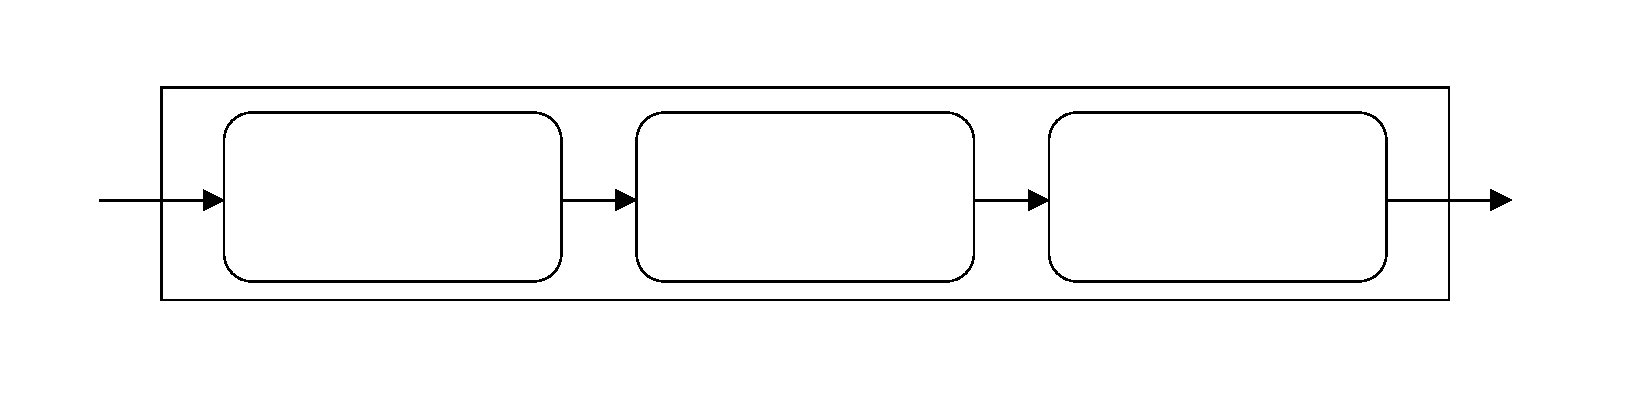
\includegraphics[width=3.0in]{figures/pipeline.eps}
%%   \caption{StreamIt pipeline}
%%   \label{fig:pipeline}
%% \end{figure}

%% \begin{scriptsize}
%% \begin{singlespace}
%% \begin{verbatim}
%% // This pipeline connects the filters scalarAdd and threeWayAverage.
%% // The parameter scalar passed to this pipeline is passed to the
%% // filter scalarAdd.
%% float -> float pipeline combinedWork(float scalar) {
%%   add scalarAdd(scalar);
%%   add threeWayAverage();
%% }
%% \end{verbatim}
%% \end{singlespace}
%% \end{scriptsize}

%%     A splitjoin arranges blocks in a parallel fashion.  The inputs to
%% a splitjoin are sent to each block in a \textit{roundrobin} or
%% \textit{duplicate} manner, and the outputs of each block are
%% joined in a roundrobin manner. Duplicate splitting means the
%% inputs to the splitjoin are copied and sent to each block, so that
%% each block receives exactly the same set of inputs.  Roundrobin
%% splitting means the inputs to the splitjoin are sent to each block
%% according to user defined weights.  For example, the first block
%% receives two inputs, the second block receives one input, the
%% third block receives two inputs.  Therefore, each block sees a
%% different set of inputs. Roundrobin joining (the only type of
%% joining permitted) means the outputs of each block are combined
%% according to user defined weights, and these represent the outputs
%% of the entire splitjoin. Blocks are listed in the order which they
%% recieve inputs using add statements. The way inputs are sent is
%% determined by using the split statement before the block list, and
%% the way outputs are recieved is determined by using the join
%% statement after the block list.

%% \begin{figure}[bthp]
%%   \centering
%%   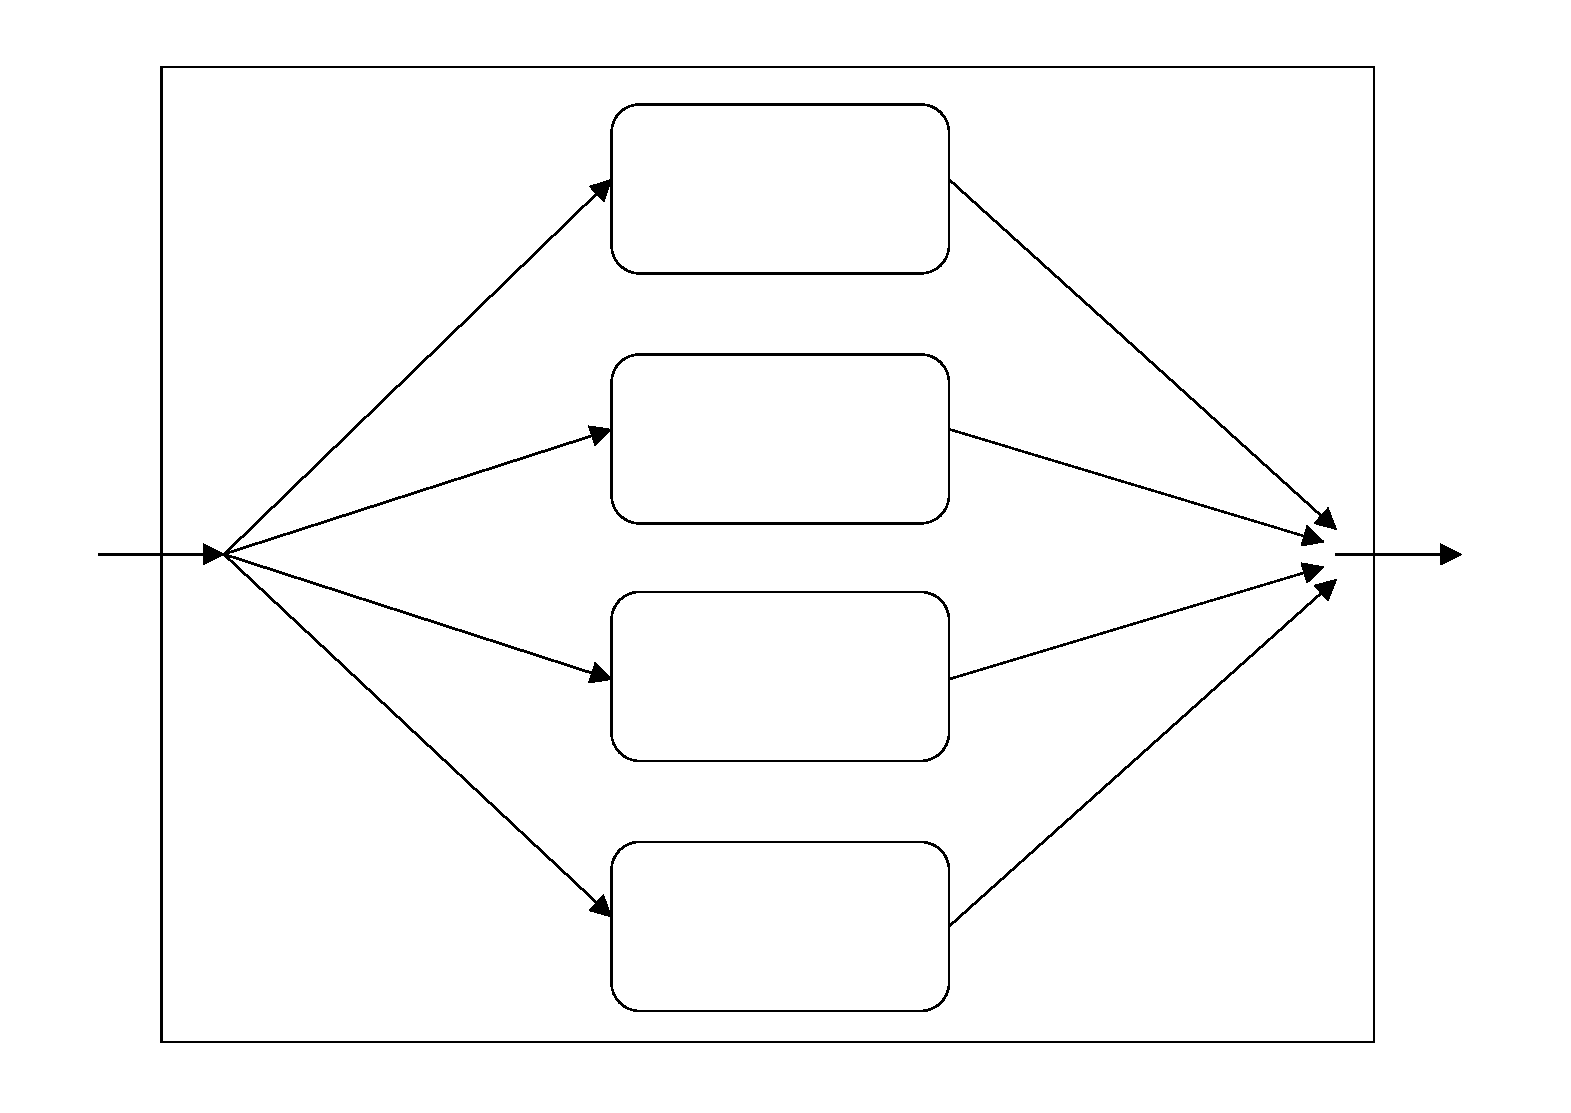
\includegraphics[width=3.0in]{figures/splitjoin.eps}
%%   \caption{StreamIt splitjoin}
%%   \label{fig:splitjoin}
%% \end{figure}

%% \begin{scriptsize}
%% \begin{singlespace}
%% \begin{verbatim}
%% // This splitjoin splits its inputs three ways.
%% // The first two inputs are sent to the first block, the next
%% // input to the second block, and the next two inputs to the third
%% // block.
%% // The outputs are collected in the following manner: three from
%% //the first block, five from the second block, and four from the
%% // third block.
%% // For every 2+1+2=5 values inputted, 3+5+4=12 values are
%% // outputted.
%% float -> float splitjoin mySplitjoin() {
%%  split roundrobin(2,1,2);
%%   add combinedWork(3.5);
%%   add combinedWork(4.5);
%%   add threeWayAverage();
%% join roundrobin(3,5,4);
%% }
%% \end{verbatim}
%% \end{singlespace}
%% \end{scriptsize}

%%     A feedback loop uses some of its output as
%% an input. It consists of a body block and a loop block. The input
%% to the entire feedback loop is combined with the output of the
%% loop block and sent to the body block, via a roundrobin joiner.
%% The output of the body block is split two ways in a roundrobin or
%% duplicate manner.  The first set of outputs is used as the output
%% of the entire feedback loop, and the second set of outputs is used
%% as the input to the loop block. Note that there must be initial
%% values enqueued on the output tape of the loop block in order for
%% the feedback loop to begin executing. The first statement in a
%% feedback loop is a join, determining how inputs are sent to the
%% body block. The body and loop blocks are listed next. The last
%% statement is a split, determining where outputs are sent from the
%% loop block.

%% \begin{figure}[bthp]
%%   \centering
%%   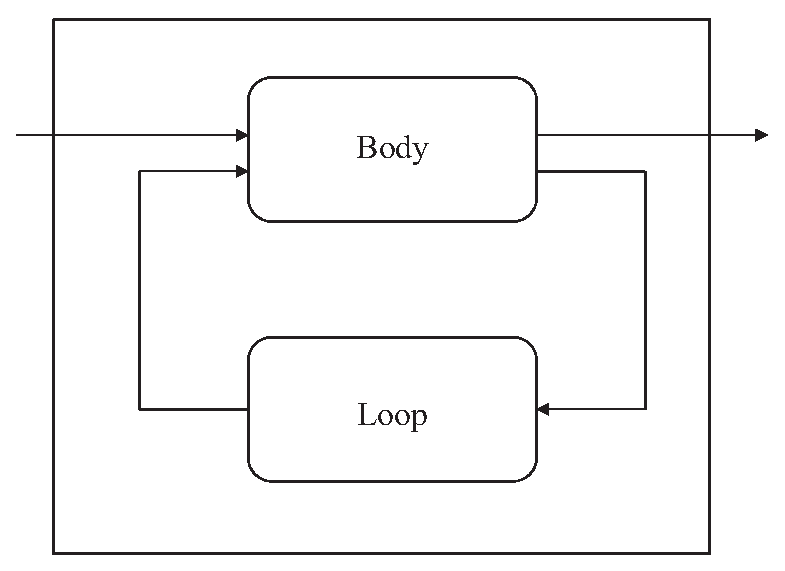
\includegraphics[width=3.0in]{figures/feedback.eps}
%%   \caption{StreamIt feedback loop}
%%   \label{fig:feedback}
%% \end{figure}

%% \begin{scriptsize}
%% \begin{singlespace}
%% \begin{verbatim}
%% // This is a feedback loop implementation of the IIR filter.
%% // The body and loop are both anonymous filters.
%% float -> float feedbackloop IIRFeedback() {
%%   join roundrobin(3,1);
%%   body float->float filter {
%%     work push 1 pop 1 peek 4 {
%%       push((peek(0)+peek(1)+peek(2))/6 + peek(3)/2);
%%       pop();
%%     }
%%   };
%%   loop float->float filter {
%%     work push 1 pop 1 peek 1 {
%%       push(pop());
%%     }
%%   };
%%   split duplicate();
%%   enqueue(0.0);
%% }
%% \end{verbatim}
%% \end{singlespace}
%% \end{scriptsize}

%%     To run a program, the StreamIt compiler finds a
%% steady-state schedule of the number of times to execute each
%% filter \cite{Karczmarek}. If such a schedule cannot be found, the
%% user created block diagram is ill-formed and could not represent a
%% real world application.

%% \mysubsection{Block Representations}

%%     The execution of a block (StreamIt or otherwise) can by
%% characterized by a single equation if the block is linear, and a
%% pair of equations if the block is state space linear. We describe
%% these terms in detail below.

%% \mysubsubsection{Linear Representations}

%%     A block is termed linear if its outputs are a linear
%% combination of its inputs plus a set of constants. In mathematical
%% terms, this relationship can be modelled by the equation
%% $\vec{\mathbf{y}} = \mathbf{D}\vec{\mathbf{u}} +
%% \vec{\mathbf{b}}$, where $\vec{\mathbf{u}}$ is a column vector
%% representing the inputs, $\mathbf{D}$ is a matrix representing the
%% weights applied to each input, $\vec{\mathbf{b}}$ is a column
%% vector representing constants added to the inputs, and
%% $\vec{\mathbf{y}}$ is a column vector representing the outputs.

%%     Suppose we have the following linear model:
%% \starteqnstar
%% \vec{\mathbf{y}} = \left [ \begin{array} {cc} 1 & 2 \\ 3 & 4 \\
%% 5 & 6 \end{array} \right ] \vec{\mathbf{u}} + \left [
%% \begin{array} {c} 7
%% \\ 8 \\ 9 \end{array}\right ]
%% \doneeqnstar

%%     It is exactly described by the following StreamIt filter:
%% \begin{scriptsize}
%% \begin{singlespace}
%% \begin{verbatim}
%% int -> int filter linearFilter() {
%%   work push 3 pop 2 peek 2 {
%%     push(1*peek(0) + 2*peek(1) + 7);
%%     push(3*peek(0) + 4*peek(1) + 8);
%%     push(5*peek(0) + 6*peek(1) + 9);
%%     pop(); pop();
%%   }
%% }
%% \end{verbatim}
%% \end{singlespace}
%% \end{scriptsize}

%%     A process for analyzing and optimizing linear StreamIt filters
%% is described in \cite{Lamb}.

  \clearpage
\mysection{State-Space Analysis}
\label{sec:statespace}

We analyze StreamIt programs at the filter level. We create a data
structure representation that fully describes a state space filter. We
parse the code of each StreamIt filter to determine whether or not it
is state space; if so we initialize a data structure, fill it with the
appropriate values through a process called \emph{extraction}, and
associate the structure with the filter. We provide a set of rules to
combine state space representations of filters in higher StreamIt
blocks---pipelines, splitjoins, and feedback loops. Such a process
results in a single state space representation for the entire block.
We also describe how to \emph{expand} a representation so that it can
be combined with blocks of mis-matching dimensions.

\mysubsection{Representation}

Our first task is to create a data structure that fully captures the
state space representation of a StreamIt filter.  We save a 
filter's number of states, push rate, and pop rate in variables which
we term $s$, $u$, and $o$, respectively. Our data structure also
contains the matrices $\mathbf{A}$, $\mathbf{B}$, $\mathbf{C}$, and
$\mathbf{D}$ with dimensions $s \times s$, $s
\times o$, $u \times s$, and $u \times o$, respectively. The
inputs to a filter are denoted as $\vec{\mathbf{u}}$ (length $o$), the
outputs as $\vec{\mathbf{y}}$ (length $u$), and the states as
$\vec{\mathbf{x}}$ (length $s$). Upon every execution of the filter,
we can calculate the outputs by the formula $\vec{\mathbf{y}} =
\mathbf{C}\vec{\mathbf{x}} +
\mathbf{D}\vec{\mathbf{u}}$, and update the state matrix by the
formula $\vec{\dot{\mathbf{x}}} = \mathbf{A}\vec{\mathbf{x}} +
\mathbf{B}\vec{\mathbf{u}}$. For convenience, we will calculate
the filter outputs before updating the state matrix. Since the
states may have initial values other than zero, we store these
values as the vector $\overrightarrow{\mathbf{initVec}}$ (length
$s$).

Since we have not included a constant term in our model, we will set
one of the state variables to be the constant $1$. This variable will
not be updated by any of the states or inputs, and its initial value
will be $1$, so it will always remain that value. Any state or output
that depends on a constant term can now refer to a multiple of the
constant state variable instead.

As long as a filter's peek rate (which we term $e$) equals its pop
rate, the data structure as currently designed can fully represent the
filter. We must include additional modifications for a filter with a
peek rate greater than its pop rate. Note that such a filter still
removes $o$ items from its input tape upon every execution, but it
accesses $e-o$ additional items on its input tape. Therefore, our
current data structure would work as long as there is some way to
access these additional items.

We solve the problem of having a peek rate greater than a pop
rate by storing $e-o$ items from the input tape in the state
vector $\vec{\mathbf{x}}$. Therefore, when a filter executes, it
can access all $e$ items it needs, $o$ items from its input vector
and $e-o$ items from its state vector. These $e-o$ states must be
updated by the inputs and themselves - the specifics are covered
in the next section. We store the number of states used for inputs
as the variable $stored$. This will be useful when combining
representations.

When the filter is executed for the first time, it will have access to
the $o$ items in the input vector, but the $e-o$ states it needs will
be uninitialized from the input tape. Therefore, we need to update the
state vector before computing the output/state update equation pair
for every filter execution. We introduce two new matrices,
$\mathbf{A_{pre}}$ and $\mathbf{B_{pre}}$ to perform this
initialization. Before the filter runs it will perform the state
update $\vec{\dot{\mathbf{x}}} =
\mathbf{A_{pre}}\vec{\mathbf{x}} +
\mathbf{B_{pre}}\vec{\mathbf{u_{pre}}}$. The initialization input
vector, $\vec{\mathbf{u_{pre}}}$, has length $o_{pre} = e-o$. For
now, $o_{pre}$ and $stored$ have the same value, but combining
filters might result in $o_{pre}$ being greater than $stored$.
$\mathbf{A_{pre}}$ is $s \times s$ and $\mathbf{B_{pre}}$ is $s
\times o_{pre}$. Note that initial assignments of the state
variables by $\overrightarrow{\mathbf{initVec}}$ are done
immediately when a filter is created, while initialization by
$\mathbf{A_{pre}}$ and $\mathbf{B_{pre}}$ is afterwards, when
there are a sufficient number ($o_{pre}$) of items on the input
tape.

Putting these pieces together, we find a full representation consists
of the push and pop rates, the number of state variables, the number
of stored inputs, the four state matrices, an initial state vector,
and possibly an initial pop rate and two initialization state
matrices. We define a state space representation $\mathrm{R}$ as the
tuple $\langle$$u$, $o$, $s$, $stored$, $\mathbf{A}$, $\mathbf{B}$,
$\mathbf{C}$, $\mathbf{D}$, $\overrightarrow{\mathbf{initVec}}$,
$\mathbf{A_{pre}}$, $\mathbf{B_{pre}}$, $o_{pre}$$\rangle$. When we
introduce a representation $\mathrm{R_i}$, each of its values in the
ordered set will be denoted with the index $i$ (for example $u_i$,
$\mathbf{A_i}$). For representations of filters that do not need the
initialization matrices, we will write $\mathbf{A_{pre}} = null$,
$\mathbf{B_{pre}} = null$, $o_{pre} = 0$. In this case, the filter
will not have any stored inputs, so $stored = 0$ as well.

Representations are initially created from StreamIt filters and
ultimately converted to StreamIt filters. Between these steps,
however, representations of the higher StreamIt block types can be
derived by combining the representations of their parts.  Therefore,
from now on we will say that a representation refers to a block rather
than a filter. The exception is in the following section, where we
discuss how to create a representation from a StreamIt filter.
% Hence we explicitly refer to a filter rather than block
%representation in that section.

\mysubsection{Extraction}

We use a simple dataflow analysis to extract the state space
representation of a filter. We symbolically execute a single iteration
of a filter's work function, maintaining a vector pair representation
for each local variable and filter field variable that is encountered
(together, these are termed program variables). If the outputs and
field variables all have vector pair representations, then the filter
is state space linear, and the vectors are used as rows of
$\mathbf{A}$, $\mathbf{B}$, $\mathbf{C}$, and $\mathbf{D}$.
%See \cite{Lamb}
%for a treatment of the linear case.

We attempt to find a vector pair
($\vec{\mathbf{v}}$,$\vec{\mathbf{w}}$) for each program variable $y$
where $y = \vec{\mathbf{v}} \cdot \vec{\mathbf{u}} +
\vec{\mathbf{w}} \cdot \vec{\mathbf{x}}$. $\vec{\mathbf{u}}$ is
the filter input vector and $\vec{\mathbf{x}}$ is the filter state
vector. When $y$ is on the left hand side of an assignment
statement, terms from the right hand side are compared with
entries from $\vec{\mathbf{u}}$ (inputs) and $\vec{\mathbf{x}}$
(states). The coefficients from terms that match are used for to
fill the corresponding entries in $\vec{\mathbf{v}}$ and
$\vec{\mathbf{w}}$, as long as they are constants. If any
coefficient is not a constant, then $y$ is non-linear.

The input vector, $\vec{\mathbf{u}}$, is defined as $[peek(e-o)
~peek(e-o+1) ~... ~peek(o-1)]$. The state vector,
$\vec{\mathbf{x}}$, holds $e-o$ variables from the input tape
($peek(0) ~... ~peek(e-o-1)$), every field variable, and a
variable for the constant 1. We do not consider local variables
for the state vector, because their values are not saved across
filter executions. 
%Therefore, their values should be resolved to
%constants at compile time. 
A field variable has the initial vector
pair ($\vec{\mathbf{0}}$,$\left [
\begin{array} {ccccc} 0 & ... & 1 & ... & 0 \end{array} \right
]$), where the 1 corresponds to the field variable itself.

If the vector pair can be found, then the program variable $y$ can be
written as a linear combination of the inputs and state variables,
with the vector pair entries representing the weights.  Then the final
assignment to state variable $x_i$ by some program variable $y_i$
indicates that the $i^{th}$ rows of $\mathbf{A}$ and $\mathbf{B}$
should be $\vec{\mathbf{w_i}}$ and $\vec{\mathbf{v_i}}$,
respectively. Similarly, the $j^{th}$ push statement using program
variable $y_j$ indicates that the $j^{th}$ rows of $\mathbf{C}$ and
$\mathbf{D}$ should be $\vec{\mathbf{w_j}}$ and $\vec{\mathbf{v_j}}$,
respectively. For the constant state variable $1$, the corresponding
rows of $\mathbf{A}$ and $\mathbf{B}$ are all zeros.

We use the same procedure in the init function to find the initial
values for each field variable. However, we do not need a vector
$\vec{\mathbf{v}}$ for the inputs, since there are no inputs to
the init function. The initial value for each stored inputs is
zero, and the initial value for the variable $1$ is one.

Finally, consider the stored input states (call them
$\vec{\mathbf{x_s}}$). They are updated by the inputs; however if
$stored > o$, then some of the input states must be updated by other
input states. In particular, the first $stored-o$ input states are
updated by the last $stored-o$ inputs, and the remaining $o$ input
states are updated by the $o$ inputs. The update is described by the
equation:
\starteqnstar
\vec{\dot{\mathbf{x_s}}} = \left [
\begin{array} {cc} \mathbf{0} & \mathbf{I} \\ \mathbf{0} &
\mathbf{0} \end{array} \right ] \vec{\mathbf{x_s}} + \left [
\begin{array} {c} \mathbf{0} \\ \mathbf{I} \end{array} \right ]
\vec{\mathbf{u}}
\doneeqnstar

We also create initialization matrices to put values from the input
tape into the input states:
\starteqnstar
\vec{\dot{\mathbf{x_s}}} = \mathbf{0} \vec{\mathbf{x_s}} +
\mathbf{I} \vec{\mathbf{u_{pre}}}
\doneeqnstar

Stored inputs are always updated as shown in the same manner.
Therefore, we will use $\mathbf{A_s}$ and $\mathbf{B_s}$ to
describe this update, where the values of these two matrices are
shown in (3.1).

\mysubsubsection{Extraction Example}

Consider another IIR filter.  Unlike the example in
Section~\ref{sec:background}, this filter uses peeking to read
elements from the tape without consuming them.

\begin{singlespace}
\small
\begin{verbatim}
float->float filter IIR() {
    float curr;  // example of a field variable
    work push 1 pop 1 peek 3 {
      float temp; // example of a local variable
      temp = (peek(0) + peek(1) + peek(2))/6;
      curr = temp + curr/2;
      push(curr);
      pop();
    }
}
\end{verbatim}
\end{singlespace}
\vspace{-16pt}

\noindent The input vector is $\left [\begin{array} {c} peek(2) \end{array}
\right]$ and the state vector is $\left [\begin{array} {c} peek(0) \\ peek(1) \\ curr \\ 1 \end{array} \right]$. The first program
variable encountered is $temp$. It is given the vector pair
($\left [ \begin{array} {c} 1/6 \end{array} \right ]$, $\left [
\begin{array} {cccc} 1/6 & 1/6 & 0 & 0 \end{array} \right ]$). The
variable $curr$, as a state variable, has an initial vector pair:
($\left [ \begin{array} {c} 0 \end{array} \right ]$, $\left
[\begin{array} {cccc} 0 & 0 & 1 & 0
\end{array} \right ]$). When $curr$ is found in an assignment
statement, it is given a new vector pair, constructed as $1$ times
the vector pair for $temp$ plus $1/2$ times the old vector pair
for $curr$: ($\left [ \begin{array} {c} 1/6 \end{array} \right ]$,
$\left [ \begin{array} {cccc} 1/6 & 1/6 & 1/2 & 0 \end{array}
\right ]$). The output is $curr$, so it is given the same vector
pair. The final pair for $curr$ represents its state update. The
stored inputs $peek(0)$, $peek(1)$ are updated as mentioned in
(3.1), and the constant $1$ is not updated. Therefore, we have:

\begin{minipage}{1.6in}
\starteqnstar
\mathbf{A} = \left [ \begin{array} {cccc} 0 & 1 & 0 & 0 \\ 0 &
0 & 0 & 0 \\ 1/6 & 1/6 & 1/2 & 0 \\ 0 & 0 & 0 & 0 \end{array}
\right ]
\doneeqnstar
\end{minipage}
\begin{minipage}{1.4in}
\starteqnstar
\mathbf{B} = \left [ \begin{array} {c} 0 \\ 1 \\ 1/6 \\ 0
\end{array} \right ]
\doneeqnstar
\end{minipage}

\begin{minipage}{1.6in}
\starteqnstar
\mathbf{C} = \left [ \begin{array} {cccc} 1/6 & 1/6 & 1/2 & 0
\end{array} \right ]
\doneeqnstar
\end{minipage}
\begin{minipage}{1.4in}
\starteqnstar
\mathbf{D} = \left [ \begin{array} {c} 1/6 \end{array} \right ]
\doneeqnstar
\end{minipage}

\hspace{1in}
\begin{minipage}{1in}
\starteqnstar
\overrightarrow{\mathbf{initVec}} = \left [ \begin{array} {c}
0 \\ 0 \\ 0 \\ 1 \end{array} \right ]
\doneeqnstar
\end{minipage}

\begin{minipage}{1.6in}
\starteqnstar
\mathbf{A_{pre}} = \left [ \begin{array} {cccc} 0 & 0 & 0 & 0 \\
0 & 0 & 0 & 0 \\ 0 & 0 & 1 & 0 \\ 0 & 0 & 0 & 1 \end{array}
\right ]
\doneeqnstar
\end{minipage}
\begin{minipage}{1in}
\starteqnstar
\mathbf{B_{pre}} = \left [ \begin{array} {cc} 1 & 0 \\ 0 & 1
\\ 0 & 0 \\ 0 & 0 \end{array} \right ]
\doneeqnstar
\end{minipage} ~\\

The pop and push rates are both one, and we have four states so $o
= 1, u = 1, s = 4$. We have two stored input states, so $o_{pre} =
2, stored = 2$.

\mysubsection{Combination}

If all blocks within a pipeline, splitjoin, or feedback loop have
state space representations, we can combine them into a single
representation using the rules developed in this section. We combine
blocks for two reasons.  First, combination can eliminate redundant
computations across blocks.  Second, combination exposes optimization
opportunities, as intra-block optimizations (described in
Section~\ref{sec:optimization}) can effectively be applied across
blocks by combining the blocks first.

\mysubsubsection{Pipeline}
\label{sec:pipeline}

Consider two blocks connected in a pipeline with representations
$\mathrm{R_1}$ and $\mathrm{R_2}$. Let $\mathrm{R}$ denote the
combined representation of the two blocks, which we are trying to
derive. Suppose the output rate of $\mathrm{R_1}$ equals the input
rate of $\mathrm{R_2}$ ($u_1 = o_2$). If this is not the case, we must
expand one or both blocks to have their input/output rates match
($u_{1\_new} = o_{2\_new} = lcm(u_1,o_2)$). Block expansion is covered
in Section~\ref{sec:expansion}. Since the output of $\mathrm{R_1}$
($y_1$) is equivalent to the input of $\mathrm{R_2}$ ($u_2$), we can
write:

\begin{minipage}{3in}
\starteqnstar
\vec{\dot{\mathbf{x_1}}} & = & \mathbf{A_1}\vec{\mathbf{x_1}} + \mathbf{B_1}\vec{\mathbf{u_1}} \\
\vec{\dot{\mathbf{x_2}}} & = & \mathbf{A_2}\vec{\mathbf{x_2}} + \mathbf{B_2}\vec{\mathbf{y_1}} \\ ~ \\
\vec{\mathbf{y_1}} & = & \mathbf{C_1}\vec{\mathbf{x_1}} + \mathbf{D_1}\vec{\mathbf{u_1}} \\
\vec{\mathbf{y_2}} & = & \mathbf{C_2}\vec{\mathbf{x_2}} +
\mathbf{D_2}\vec{\mathbf{y_1}}
\doneeqnstar
\end{minipage} ~\\

Substituting for $\vec{\mathbf{y_1}}$ we get:
\starteqnstar
\vec{\dot{\mathbf{x_2}}} & = & \mathbf{A_2}\vec{\mathbf{x_2}} + \mathbf{B_2}(\mathbf{C_1}\vec{\mathbf{x_1}} + \mathbf{D_1}\vec{\mathbf{u_1}}) \\
\vec{\mathbf{y_2}} & = & \mathbf{C_2}\vec{\mathbf{x_2}} +
\mathbf{D_2}(\mathbf{C_1}\vec{\mathbf{x_1}} +
\mathbf{D_1}\vec{\mathbf{u_1}})
\doneeqnstar

Which simplifies to:
\starteqnstar
\vec{\dot{\mathbf{x_2}}} & = & \mathbf{A_2}\vec{\mathbf{x_2}} + \mathbf{B_2}\mathbf{C_1}\vec{\mathbf{x_1}} + \mathbf{B_2}\mathbf{D_1}\vec{\mathbf{u_1}} \\
\vec{\mathbf{y_2}} & = & \mathbf{C_2}\vec{\mathbf{x_2}} +
\mathbf{D_2}\mathbf{C_1}\vec{\mathbf{x_1}} +
\mathbf{D_2}\mathbf{D_1}\vec{\mathbf{u_1}}
\doneeqnstar

Let $\vec{\mathbf{x}} = \left [ \begin{array} {c} \vec{\mathbf{x_1}} \\
\vec{\mathbf{x_2}} \end{array} \right ]$, $\vec{\mathbf{u}} =
\vec{\mathbf{u_1}}$ (the input to the entire pipeline), and
$\vec{\mathbf{y}} = \vec{\mathbf{y_2}}$ (the output of the entire
pipeline). The equations relating $\vec{\mathbf{x}}$,
$\vec{\mathbf{u}}$, and $\vec{\mathbf{y}}$ are:
\starteqnstar
\vec{\dot{\mathbf{x}}} & = & \mathbf{A}\vec{\mathbf{x}} + \mathbf{B}\vec{\mathbf{u}} \\
\vec{\mathbf{y}} & = & \mathbf{C}\vec{\mathbf{x}} + \mathbf{D}\vec{\mathbf{u}}
\doneeqnstar ~ \\ \vspace{-36pt} ~ \\
\starteqnstar
\mathbf{A} = \left [ \begin{array} {cc} \mathbf{A_1} &
\mathbf{0} \\ \mathbf{B_2}\mathbf{C_1} & \mathbf{A_2} \end{array} \right ] &~&
\mathbf{B} = \left [ \begin{array} {c} \mathbf{B_1} \\ \mathbf{B_2}\mathbf{D_1} \end{array} \right ] \\ ~&~&~ \\
\mathbf{C} = \left [ \begin{array} {cc} \mathbf{D_2}\mathbf{C_1} & \mathbf{C_2} \end{array} \right ] &~&
\mathbf{D} = \mathbf{D_2}\mathbf{D_1}
\doneeqnstar

The input to the pipeline is identical to the input to $\mathrm{R_1}$,
and the output of the pipeline is identical to the output of
$\mathrm{R_2}$. Furthermore, the states of the pipeline are the states
of the first block appended to the states of the second
block. Therefore, $u = u_2$, $o = o_1$, $s = s_1 + s_2$,
$\overrightarrow{\mathbf{initVec}} = \left [ \begin{array} {c}
\overrightarrow{initVec_1} \\ \overrightarrow{initVec_2}
\end{array} \right ]$.

If both blocks do not have initialization matrices, then the entire
pipeline does not need initialization matrices, so $\mathbf{A_{pre}} =
null$, $\mathbf{B_{pre}} = null$, $o_{pre} = 0$, $stored = 0$. If only
the first block has initialization matrices, then we want to
initialize the states in the pipeline corresponding to the first block
while keeping the states corresponding to the second block
unchanged. Therefore:
\starteqnstar
\mathbf{A_{pre}} = \left [ \begin{array} {cc}
\mathbf{A_{pre1}} & \mathbf{0} \\ \mathbf{0} & \mathbf{I} \end{array} \right ] ~~~~~
\mathbf{B_{pre}} = \left [ \begin{array} {c} \mathbf{B_{pre1}} \\ \mathbf{0} \end{array} \right ]
\doneeqnstar ~ \\ \vspace{-36pt} ~ \\
\starteqnstar
o_{pre} = o_{pre1} ~~~~~
stored = stored_1
\doneeqnstar

If the second block has initialization matrices, we must run the first
block enough times to provide the necessary inputs to initialize the
second block. However, this might result in the first block providing
extra initial inputs to the second block. In that case, we must change
the representation of the second block to increase its number of
stored inputs.  A full description of this case appears
in~\cite{Agrawal04}.

%%  (the way to do this is
%% covered in Section 3.4.2). Suppose this is done and the first
%% block must run $n$ times (along with its initialization matrices,
%% if it has them) to initialize the second block. Denote
%% $\mathbf{{A_1}^e}$, $\mathbf{{B_1}^e}$, $\mathbf{{C_1}^e}$, and
%% $\mathbf{{D_1}^e}$ as the matrices that describe running the first
%% block $n$ times (see Equations (3.6)-(3.9)). Then the
%% initialization of the entire pipeline is derived by combining
%% these matrices with $\mathbf{A_{pre2}}$, $\mathbf{B_{pre2}}$ just
%% as the $\mathbf{A}$, $\mathbf{B}$, $\mathbf{C}$, and $\mathbf{D}$
%% matrices are combined for the two blocks:
%% \starteqnstar
%% \mathbf{A_{pre}} & = & \left [ \begin{array} {cc}
%% \mathbf{{A_1}^e} & \mathbf{0} \\
%% \mathbf{B_{pre2}} \mathbf{{C_1}^e} & \mathbf{A_{pre2}} \end{array} \right ] \\
%% \mathbf{B_{pre}} & = & \left [ \begin{array} {c}
%% \mathbf{{B_1}^e} \\ \mathbf{B_{pre2}} \mathbf{{D_1}^e} \\ \end{array} \right ] \\
%% o_{pre} & = & o_{pre1} + n*o_1 \\
%% stored & = & stored_1
%% \doneeqnstar

If there are more than two blocks in a pipeline, we collapse the
pipeline in the following manner: combine the first two blocks to get
one block representation, combine this with the third block, etc.

\mysubsubsection{Splitjoin and Feedback Loop}

The combination rules for splitjoins and feedback loops are somewhat
involved, and we omit them due to space considerations.  An important
benefit of a linear state space representation over a linear
representation is that feedback loops can be collapsed; the items on
the feedback path become states in the combined block.  A thorough
treatment of these cases appears in~\cite{Agrawal04}.

%%     There are two types of splitjoins - those with roundrobin and
%% duplicate splitters. In order to collapse the branches of a
%% splitjoin to a single representation, we need the splitjoin to
%% have a duplicate splitter, because then the representation in each
%% branch accesses the same inputs. Therefore, for roundrobin
%% splitjoins we first detail a procedure to convert to a duplicate
%% splitjoin. Then we describe how to create a representation of a
%% duplicate splitjoin.

%% \subsubsubsection{Conversion from roundrobin to duplicate splitjoin}

%%     Suppose the roundrobin splitjoin has $k$ branches and let $w_i$ and
%% $\mathrm{M_i}$ denote the splitter weight and state space
%% representation, respectively, on the $i^{th}$ branch. In each
%% branch $i$ we add a filter with representation $\mathrm{L_i}$ that
%% outputs to $\mathrm{M_i}$ in a pipeline format. Since the
%% splitjoin now has a duplicate splitter, $\mathrm{M_i}$ receives
%% every input element to the entire splitjoin. In order to exactly
%% simulate the original roundrobin splitter, $\mathrm{M_i}$ should
%% only see $w_i$ elements for every $\sum_{j=1}^{k} w_j$ input
%% elements to the splitjoin. Therefore, we make $\mathrm{L_i}$ input
%% $\sum_{j=1}^{k} w_j$ elements and output $w_i$ elements. In
%% particular, $\mathrm{L_i}$ ignores the first $\sum_{j=1}^{i-1}
%% w_j$ inputs (which correspond to inputs to the previous branches),
%% outputs the next $w_i$ inputs (which correspond to inputs to the
%% $i^{th}$ branch), and ignores the remaining $\sum_{j=i+1}^{k} w_j$
%% inputs\footnote{In DSP terminology, $\mathrm{L_i}$ is called a
%% downsampler.} (which correspond to inputs to the later branches).

%%     The values for $\mathrm{L_i}$ are $o = \sum_{j=1}^{k} w_j$, $u = w_i$,
%% $s = 1$, $\mathbf{A} = \mathbf{0}$, $\mathbf{B} = \mathbf{0}$,
%% $\mathbf{C} = \mathbf{0}$, $\mathbf{D} = \left [ \begin{array}
%% {ccc} \mathbf{0} & \mathbf{I} & \mathbf{0} \end{array} \right ]$,
%% $\overrightarrow{\mathbf{initVec}} = \vec{\mathbf{0}}$,
%% $\mathbf{A_{pre}}, \mathbf{B_{pre}} = null$, $o_{pre} = 0$,
%% $stored = 0$. We use one state in the representation, even though
%% none are needed, to make combinations of representations simpler.
%% Once $\mathrm{L_i}$ is created, it can be combined with
%% $\mathrm{M_i}$ to form a single representation (call it
%% $\mathrm{R_i}$).

%% \subsubsubsection{Collapsing duplicate splitjoins}

%%     Let $\mathrm{R}$ be the representation for the entire
%% splitjoin, $\mathrm{R_i}$ be the representation on the $i^{th}$
%% branch, $k$ be the number of branches. In order to combine the
%% branch representations, we must derive a steady-state execution of
%% the entire splitjoin. Denote the joiner weight of each branch $i$
%% as $w_i$ (note that we used $w_i$ earlier to denote a splitter
%% weight). Each branch outputs $u_i$ items but $w_i$ items from that
%% branch are needed to execute the splitjoin once. $\mathrm{R_i}$
%% can be expanded to output $lcm(u_i,w_i)$ items, which would result
%% in $\frac{lcm(u_i,w_i)}{w_i}$ splitjoin executions. This means we
%% must execute the splitjoin a multiple of
%% $\frac{lcm(u_1,w_1)}{w_1}$ times to satisfy the constraints of the
%% first branch, a multiple of $\frac{lcm(u_2,w_2)}{w_2}$ times to
%% satisfy the constraints of the second branch, etc. Therefore, we
%% shall construct $\mathrm{R}$ to execute the splitjoin
%% $lcm(\frac{lcm(u_1,w_1)}{w_1},\frac{lcm(u_2,w_2)}{w_2},...,\frac{lcm(u_k,w_k)}{w_k})$
%% times. Call this value $E$. Each representation $\mathrm{R_i}$
%% must output $w_i * E$ elements, so $\mathrm{R_i}$ must be expanded
%% $\frac{w_i * E}{u_i}$ times.

%%     After these expansions, each branch representation  should now
%% have the same input rate $o_i$. If not, the splitjoin is
%% ill-formed and cannot be compiled by StreamIt. Since these
%% representations will be combined, we need each to have the same
%% number of stored inputs and the same initial pop rate. To satisfy
%% both constraints, we increase the number of stored inputs in each
%% representation to the value $max(stored_i,o_{prei})$ over all $i$.

%%     Now that the branch representations have been standardized,
%% they can be combined to a single representation. The stored input
%% states in each representation evolve in the same manner, so only
%% one set of them is needed for the entire splitjoin representation.
%% Let $\vec{\mathbf{x_i}} = \left [ \begin{array} {c}
%% \vec{\mathbf{x_{is}}} \\ \vec{\mathbf{x_{ir}}} \end{array} \right
%% ]$, where $\vec{\mathbf{x_{is}}}$ and $\vec{\mathbf{x_{ir}}}$ are
%% the stored input states and remaining states of $\mathrm{R_i}$,
%% respectively. For each representation $i$ denote the state space
%% equation pair as:
%% \starteqnstar
%% \left [ \begin{array} {c} \vec{\dot{\mathbf{x_{is}}}} \\
%% \vec{\dot{\mathbf{x_{ir}}}} \end{array} \right ] & = & \left [
%% \begin{array} {cc} \mathbf{A_{is}} & \mathbf{0} \\
%% \mathbf{A_{irs}} & \mathbf{A_{irr}} \end{array} \right ] \left [
%% \begin{array} {c} \vec{\mathbf{x_{is}}} \\ \vec{\mathbf{x_{ir}}}
%% \end{array} \right ] +  \left [ \begin{array} {c} \mathbf{B_{is}}
%% \\ \mathbf{B_{ir}} \end{array} \right ] \vec{\mathbf{u}} \\
%% \vec{\mathbf{y}} & = & \left [ \begin{array} {cc} \mathbf{C_{is}}
%% & \mathbf{C_{ir}} \end{array} \right ] \left [ \begin{array} {c}
%% \vec{\mathbf{x_{is}}} \\ \vec{\mathbf{x_{ir}}} \end{array} \right
%% ] + \mathbf{D} \vec{\mathbf{u}}
%% \doneeqnstar

%%     Since the stored input states in each representation are
%% equivalent, we set them to be $\vec{\mathbf{x_s}}$, and set their
%% corresponding matrix blocks to be $\mathbf{A_s}$ and
%% $\mathbf{B_s}$. Let $\vec{\mathbf{x}} = \left [ \begin{array} {c}
%% \vec{\mathbf{x_{s}}} \\ \vec{\mathbf{x_{1r}}} \\
%% \vec{\mathbf{x_{2r}}} \\ ... \\ \vec{\mathbf{x_{kr}}} \end{array}
%% \right ]$. The states $\vec{\mathbf{x_{ir}}}$ evolve separately,
%% so:
%% \starteqnstar
%% \mathbf{A} & = & \left [ \begin{array} {ccccc} \mathbf{A_s} &
%% \mathbf{0} & \mathbf{0} & ... & \mathbf{0} \\ \mathbf{A_{1rs}} &
%% \mathbf{A_{1rr}} & \mathbf{0} & ... & \mathbf{0} \\
%% \mathbf{A_{2rs}} & \mathbf{0} & \mathbf{A_{2rr}} & ... & \mathbf{0}
%% \\ ... & ... & ... & ... \\ \mathbf{A_{krr}} & \mathbf{0} &
%% \mathbf{0} & ... & \mathbf{A_{krs}} \end{array} \right ] \\
%% \mathbf{B} & = & \left [ \begin{array} {c} \mathbf{B_s} \\ \mathbf{B_{1r}} \\
%% \mathbf{B_{2r}} \\ ... \\ \mathbf{B_{kr}} \end{array} \right ]
%% \doneeqnstar

%%     Similarly for the initialization matrices we have:
%% \starteqnstar
%% \mathbf{A_{pre}} & = & \left [ \begin{array} {ccccc} \mathbf{0} &
%% \mathbf{0} & \mathbf{0} & ... & \mathbf{0} \\
%% \mathbf{0} & \mathbf{A_{pre1rr}} & \mathbf{0} & ... & \mathbf{0} \\
%% \mathbf{0} & \mathbf{0} & \mathbf{A_{pre2rr}} & ... & \mathbf{0} \\
%% ... & ... & ... & ... & ... \\ \mathbf{0} & \mathbf{0} &
%% \mathbf{0} & ... & \mathbf{A_{prekrr}} \end{array} \right ] \\
%% \mathbf{B_{pre}} & = & \left [ \begin{array} {c} \mathbf{B_{pres}} \\
%% \mathbf{B_{pre1r}} \\ \mathbf{B_{pre2r}} \\ ... \\
%% \mathbf{B_{prekr}} \end{array} \right ]
%% \doneeqnstar

%%     These equations are simpler because $\mathbf{A_{pres}} =
%% \mathbf{0}$ and $\mathbf{A_{preirs}} = \mathbf{0}$.

%%     In order to simulate the roundrobin nature of the joiner,
%% we must output $w_1$ items from $\mathrm{R_1}$, then $w_2$ items
%% from $\mathrm{R_2}$, up to $w_k$ items from $\mathrm{R_k}$, and
%% repeat this process $E$ times (because we are running the
%% splitjoin $E$ times). Let $\mathbf{C_i} = \left [
%% \begin{array} {cc} \mathbf{C_{is1}} & \mathbf{C_{ir1}} \\
%% \mathbf{C_{is2}} & \mathbf{C_{ir2}} \\ ... & ... \\
%% \mathbf{C_{isexecutions}} & \mathbf{C_{irexecutions}} \end{array}
%% \right ]$, where $\left [ \begin{array} {cc} \mathbf{C_{isj}} &
%% \mathbf{C_{irj}} \end{array} \right ]$ is $w_i \times s_i$. Let
%% $\mathbf{D_i} = \left [
%% \begin{array} {c} \mathbf{D_{i1}} \\ \mathbf{D_{i2}} \\ ... \\
%% \mathbf{D_{iexecutions}} \end{array} \right ]$, where
%% $\mathbf{D_{ij}}$ is $w_i \times o$. Then we have:
%% \starteqnstar
%% \mathbf{C} & = & \left [ \begin{array} {ccccc} \mathbf{C_{1s1}} &
%% \mathbf{C_{1r1}} & \mathbf{0} & ... & \mathbf{0} \\
%% \mathbf{C_{2s1}} & \mathbf{C_{2r1}} & \mathbf{0} & ... &
%% \mathbf{0} \\ ... & ... & ... & ... & ... \\ \mathbf{C_{ks1}} &
%% \mathbf{0} & \mathbf{0} & ... & \mathbf{C_{kr1}} \\ ... & ... & ... & ... & ... \\
%% \mathbf{C_{1sk}} & \mathbf{C_{1rk}} & \mathbf{0} & ... & \mathbf{0} \\
%% \mathbf{C_{2sk}} & \mathbf{C_{2rk}} & \mathbf{0} & ... & \mathbf{0} \\
%% ... & ... & ... & ... \\ \mathbf{C_{ksk}} & \mathbf{0} & \mathbf{0} & ... & \mathbf{C_{krk}}
%% \end{array} \right ] \\
%% \mathbf{D} & = & \left [ \begin{array} {c} \mathbf{D_{11}} \\
%% \mathbf{D_{21}} \\ ... \\ \mathbf{D_{k1}} \\ ... \\ \mathbf{D_{1k}} \\
%% \mathbf{D_{2k}} \\ ... \\ \mathbf{D_{kk}} \end{array} \right ]
%% \doneeqnstar

%%     We have derived $\mathbf{A}$, $\mathbf{B}$, $\mathbf{C}$,
%% $\mathbf{D}$, $\mathbf{A_{pre}}$, and $\mathbf{B_{pre}}$. As
%% mentioned previously, all the pop rates are equal so $o = o_1$.
%% Additionally, all the initial pop rates and stored inputs are
%% equal, so $o_{pre} = o_{pre1}$ and $stored = o_{pre1}$. The
%% splitjoin runs $E$ times, hence $u = E * \sum_{j=1}^{k} w_j$. The
%% states of the entire representation are the non-stored input
%% states of each branch representation concatenated along with one
%% set of the stored input states. Let $s_{ir}$ be the number of
%% non-stored input states in representation $i$ and let
%% $\overrightarrow{\mathbf{initVec_{ir}}}$ be the initial values of
%% these states. Then $s = stored + \sum_{j=1}^{k} s_{jr}$ and
%% $\overrightarrow{\mathbf{initVec}} =
%% \left [ \begin{array} {c} \vec{\mathbf{0}} \\ \overrightarrow{\mathbf{initVec_{1r}}} \\
%% \overrightarrow{\mathbf{initVec_{2r}}} \\ ... \\
%% \overrightarrow{\mathbf{initVec_{kr}}} \end{array} \right ]$.

%% \mysubsubsection{Feedback Loop}

%%     Recall that a feedback loop has a loop block and a body block.
%% Outputs from the body block and inputs to the entire feedback loop
%% are combined via a joiner to form the inputs to the loop block.
%% Outputs from the loop block are used as outputs of the entire
%% feedback loop and inputs of the loop block via a splitter.

%%     Let the loop block have representation $\mathrm{R_1}$, the body
%% block have representation $\mathrm{R_2}$, and the entire feedback
%% loop have representation $\mathrm{R}$. If the splitter is a
%% roundrobin one, we convert it to a duplicate one by adding the
%% appropriate downsamplers to the output branches, as described in
%% Section 3.3.2. The output branches of a feedback loop splitter
%% lead to the loop block and the output of the entire feedback loop.
%% Therefore, one downsampler must be placed before the loop block in
%% a pipeline format, and one downsampler must be placed after the
%% feedback loop in a pipeline format. The first downsampler and loop
%% block is combined to form a new loop block. The second downsampler
%% can be combined with the feedback loop after the feedback loop's
%% representation is computed.

%%     As in the case of a splitjoin, we must derive a steady-state
%% execution of the entire feedback loop in order to combine the loop
%% and body blocks. First we match the output rate of the body block
%% ($o_2$) with the input rate of the loop block ($u_1$) by expanding
%% the two representations appropriately. Now consider the roundrobin
%% joiner, and let $w_1$, $w_2$ be the weights on the branches from
%% the loop block and input to the body block, respectively. The loop
%% block outputs $u_1$ items, but $w_1$ items are needed to run the
%% feedback loop once. Therefore, the loop block can be expanded to
%% output $lcm(u_1,w_1)$ items, which would result in
%% $\frac{lcm(u_1,w_1)}{w_1}$ feedback loop executions. Call this
%% value $E$. The loop block is expanded to run
%% $\frac{lcm(u_1,w_1)}{u_1}$ times, and the body block is expanded
%% by this amount as well, since we still want the output rate of the
%% body block to equal the input rate of the loop block. Since the
%% feedback loop runs $E$ times, the body block receives $E*(w_1 +
%% w_2)$ inputs, which should equal the input rate of the expanded
%% body block. If not, the feedback loop is ill-formed.

%%     Once the above expansions are implemented, the feedback loop
%% is run by executing the loop and body blocks alternately. However,
%% the loop block depends on outputs from the body block, and the
%% body block depends on outputs from the loop block. In order to
%% begin execution of the entire feedback loop, there must be items
%% enqueued on the output tape of the loop block. The minimal number
%% of enqueued items is $u_1$, the output rate of the loop block.
%% However, there can be more enqueued items. We create a new
%% representation $\mathrm{R_3}$ that stores the enqueued values.
%% Upon each execution $\mathrm{R_3}$ inputs $u_1$ items from the
%% loop block and outputs $u_1$ items to the body block. It has one
%% state for each enqueued item. The equations for $\mathrm{R_3}$
%% are:
%% \starteqnstar
%% \vec{\dot{\mathbf{x_3}}} & = & \left [ \begin{array} {cc}
%% \mathbf{0} & \mathbf{I} \\ \mathbf{0} & \mathbf{0} \end{array} \right ]
%% \vec{\mathbf{x_3}} + \left [ \begin{array} {c} \mathbf{0} \\ \mathbf{I}
%% \end{array} \right ] \vec{\mathbf{u_3}} \\
%% \vec{\mathbf{y_3}} & = & \left [ \begin{array} {c} \mathbf{I} \\
%% \mathbf{0} \end{array} \right ] \vec{\mathbf{x_1}}
%% \doneeqnstar

%%     $\mathrm{R_3}$ does not have initialization matrices, and
%% $\overrightarrow{\mathbf{initVec_3}}$ is assigned the enqueued
%% values.

%%     Note that the output $\vec{\mathbf{y_3}}$ does not depend on
%% the input $\vec{\mathbf{u_3}}$. This is the key to starting the
%% feedback loop: $\mathrm{R_3}$ outputs first, the body block uses
%% these outputs along with inputs to the entire feedback loop to
%% execute and produce outputs, the loop body uses these outputs to
%% execute and produce outputs, $\mathrm{R_3}$ uses these outputs to
%% execute and produce outputs, etc.

%% \begin{figure}[bthp]
%%   \centering
%%   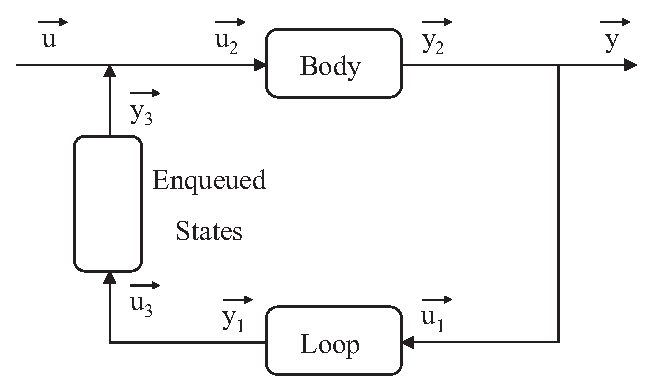
\includegraphics[width=3.0in]{figures/feedback2.eps}
%%   \caption{Labelled feedback loop}
%%   \label{fig:feedback2}
%% \end{figure}

%%     From figure \ref{fig:feedback2} it is apparent that $\vec{\mathbf{u_3}} =
%% \vec{\mathbf{y_1}}$, $\vec{\mathbf{y}} = \vec{\mathbf{y_2}} =
%% \vec{\mathbf{u_1}}$, and $\vec{\mathbf{u_2}}$ is composed of
%% $\vec{\mathbf{u}}$ and $\vec{\mathbf{u_3}}$. We can write the
%% equations for the body block as:
%% \starteqnstar
%% \vec{\dot{\mathbf{x_2}}} & = & \mathbf{A_2} \vec{\mathbf{x_2}} +
%% \mathbf{B_2} \vec{\mathbf{u_2}} = \mathbf{A_2}\vec{\mathbf{x_2}} +
%% \mathbf{B_{2\_1}} \vec{\mathbf{u}} + \mathbf{B_{2\_2}}
%% \vec{\mathbf{y_3}} = \mathbf{A_2}\vec{\mathbf{x_2}} +
%% \mathbf{B_{2\_1}} \vec{\mathbf{u}} + \mathbf{B_{2\_2}}
%% \mathbf{C_3} \vec{\mathbf{x_3}} \\
%% \vec{\mathbf{y_2}} & = & \mathbf{C_2} \vec{\mathbf{x_2}} +
%% \mathbf{D_2} \vec{\mathbf{u_2}} = \mathbf{C_2}\vec{\mathbf{x_2}} +
%% \mathbf{D_{2\_1}} \vec{\mathbf{u}} + \mathbf{D_{2\_2}}
%% \vec{\mathbf{y_3}} = \mathbf{C_2}\vec{\mathbf{x_2}} +
%% \mathbf{D_{2\_1}} \vec{\mathbf{u}} + \mathbf{D_{2\_2}}
%% \mathbf{C_3} \vec{\mathbf{x_3}}
%% \doneeqnstar

%%     Since $\vec{\mathbf{y}} = \vec{\mathbf{y_2}}$, we have written
%% the output of the feedback loop and the update for
%% $\vec{\mathbf{x_2}}$ in terms of the input to the feedback loop
%% and the state vectors. For the updates to $\vec{\mathbf{x_1}}$ and
%% $\vec{\mathbf{x_3}}$ we can write:
%% \starteqnstar
%% \vec{\dot{\mathbf{x_1}}} & = & \mathbf{A_1} \vec{\mathbf{x_1}} +
%% \mathbf{B_1} \vec{\mathbf{u_1}} = \mathbf{A_1}\vec{\mathbf{x_1}} +
%% \mathbf{B_1} \vec{\mathbf{y}} =  \mathbf{A_1}\vec{\mathbf{x_1}} +
%% \mathbf{B_1}(\mathbf{C_2}\vec{\mathbf{x_2}} + \mathbf{D_{2\_1}}
%% \vec{\mathbf{u}} + \mathbf{D_{2\_2}} \mathbf{C_3}
%% \vec{\mathbf{x_3}}) \\
%% & = & \mathbf{A_1}\vec{\mathbf{x_1}} +
%% \mathbf{B_1}\mathbf{C_2}\vec{\mathbf{x_2}} + \mathbf{B_1}
%% \mathbf{D_{2\_1}} \vec{\mathbf{u}} + \mathbf{B_1}
%% \mathbf{D_{2\_2}} \mathbf{C_3} \vec{\mathbf{x_3}} \\ \\
%% \vec{\dot{\mathbf{x_3}}} & = & \mathbf{A_3} \vec{\mathbf{x_3}} +
%% \mathbf{B_3} \vec{\mathbf{u_3}} = \mathbf{A_3}\vec{\mathbf{x_3}} +
%% \mathbf{B_3} \vec{\mathbf{y_1}} =  \mathbf{A_3}\vec{\mathbf{x_3}}
%% + \mathbf{B_3}(\mathbf{C_1}\vec{\mathbf{x_1}} + \mathbf{D_1}
%% \vec{\mathbf{u_1}}) \\
%% & = & \mathbf{A_3}\vec{\mathbf{x_3}} +
%% \mathbf{B_3}(\mathbf{C_1}\vec{\mathbf{x_1}} +
%% \mathbf{D_1}\vec{\mathbf{y}}) = \mathbf{A_3}\vec{\mathbf{x_3}} +
%% \mathbf{B_3}(\mathbf{C_1}\vec{\mathbf{x_1}} +
%% \mathbf{D_1}(\mathbf{C_2}\vec{\mathbf{x_2}} + \mathbf{D_{2\_1}}
%% \vec{\mathbf{u}} + \mathbf{D_{2\_2}} \mathbf{C_3}
%% \vec{\mathbf{x_3}})) \\
%% & = & \mathbf{A_3}\vec{\mathbf{x_3}} +
%% \mathbf{B_3}\mathbf{C_1}\vec{\mathbf{x_1}} +
%% \mathbf{B_3}\mathbf{D_1}\mathbf{C_2}\vec{\mathbf{x_2}} +
%% \mathbf{B_3}\mathbf{D_1}\mathbf{D_{2\_1}} \vec{\mathbf{u}} +
%% \mathbf{B_3}\mathbf{D_1}\mathbf{D_{2\_2}} \mathbf{C_3}
%% \vec{\mathbf{x_3}}
%% \doneeqnstar

%%     For the input and output rates we have $o = E * w_2$
%% and $u = u_2$. We use the states of all three representations, so
%% $s = s_1 + s_2 + s_3$ and $\overrightarrow{\mathbf{initVec}} =
%% \left [ \begin{array} {c} \overrightarrow{\mathbf{initVec_1}} \\
%% \overrightarrow{\mathbf{initVec_2}} \\
%% \overrightarrow{\mathbf{initVec_3}} \end{array} \right ]$. For
%% simplicity, we do not consider a loop or body block with
%% initialization matrices.

\mysubsection{Expanding a Representation}
\label{sec:expansion}

We may want to run a block multiple times in order to properly combine
it with other blocks. For example, suppose block $B_1$ inputs three
items and outputs two items, and block $B_2$ inputs five items and
outputs seven items. In order to combine these blocks in a pipeline,
$B_1$ must run five times (in order to output ten items) and $B_2$
must run two times (in order to input ten items). Therefore, we need
to have a method to expand a representation so that it models a block
running multiple times, rather than once.

Consider the state space equation pair, where $\vec{\mathbf{u_1}}$ and
$\vec{\mathbf{y_1}}$ are the first set of inputs and outputs, and
$\vec{\mathbf{x}}$ is the original state vector:
\starteqnstar
\vec{\dot{\mathbf{x}}} & = & \mathbf{A}\vec{\mathbf{x}} + \mathbf{B}\vec{\mathbf{u_1}} \\
\vec{\mathbf{y_1}} & = & \mathbf{C}\vec{\mathbf{x}} +
\mathbf{D}\vec{\mathbf{u_1}}
\doneeqnstar

If we run the block again, the equation pair in terms of the
original state vector $\vec{\mathbf{x}}$ and the next set of
inputs and outputs ($\vec{\mathbf{u_2}}$ and $\vec{\mathbf{y_2}}$)
is:
\starteqnstar
\vec{\dot{\mathbf{x}}} & = & \mathbf{A}(\mathbf{A}\vec{\mathbf{x}}
+
\mathbf{B}\vec{\mathbf{u_1}}) + \mathbf{B}\vec{\mathbf{u_2}} \\
\vec{\mathbf{y_2}} & = & \mathbf{C}(\mathbf{A}\vec{\mathbf{x}} +
\mathbf{B}\vec{\mathbf{u_1}}) + \mathbf{D}\vec{\mathbf{u_2}}
\doneeqnstar
\noindent Simplifying yields:
\starteqnstar
\vec{\dot{\mathbf{x}}} & = & \mathbf{A}^2\vec{\mathbf{x}} +
\mathbf{AB}\vec{\mathbf{u_1}} + \mathbf{B}\vec{\mathbf{u_2}} \\
\vec{\mathbf{y_2}} & = & \mathbf{CA}\vec{\mathbf{x}} +
\mathbf{CB}\vec{\mathbf{u_1}} + \mathbf{D}\vec{\mathbf{u_2}}
\doneeqnstar

Let $\vec{\mathbf{u}}$ be the combined input vector ($\vec{\mathbf{u}}
= \left [ \begin{array} {c} \vec{\mathbf{u_1}}
\\ \vec{\mathbf{u_2}} \end{array} \right ]$) and $\vec{\mathbf{y}}$ be the combined output vector
($\vec{\mathbf{y}} = \left [ \begin{array} {c} \vec{\mathbf{y_1}}
\\ \vec{\mathbf{y_2}} \end{array} \right ]$). The representation in terms of these two
vectors is:
\starteqnstar
\vec{\dot{\mathbf{x}}} & = & \mathbf{A_2}\vec{\mathbf{x}} + \mathbf{B_2}\vec{\mathbf{u}} \\
\vec{\mathbf{y}} & = & \mathbf{C_2}\vec{\mathbf{x}} + \mathbf{D_2}\vec{\mathbf{u}}
\doneeqnstar ~ \\ \vspace{-36pt} ~ \\
\starteqnstar
\mathbf{A_2} = \mathbf{A}^2 ~~~~~
\mathbf{B_2} = \left [ \begin{array} {cc} \mathbf{AB} & \mathbf{B} \end{array} \right ]  \\ ~ \\
\mathbf{C_2} = \left [ \begin{array} {c} \mathbf{C} \\
\mathbf{CA} \end{array} \right ] ~~~~~
\mathbf{D_2} = \left [ \begin{array} {cc} \mathbf{D} & \mathbf{0} \\
\mathbf{CB} & \mathbf{D} \end{array} \right ]
\doneeqnstar
This new representation corresponds to a block that upon every
execution runs the old block twice. By induction, a general formula
for running a block n times is:
\starteqnstar
\mathbf{A_n} = \mathbf{A}^n ~~~~~
\mathbf{B_n} = \left [ \begin{array} {ccccc} \mathbf{A}^{n-1}
\mathbf{B} & \mathbf{A}^{n-2} \mathbf{B} & ...  & \mathbf{AB} &
\mathbf{B} \end{array} \right ]
\doneeqnstar
\starteqnstar
\mathbf{C_n} = \left [ \begin{array} {c} \mathbf{C} \\
\mathbf{CA} \\
... \\
\mathbf{CA^{n-2}} \\
\mathbf{CA^{n-1}} \end{array} \right ]~~~~~~~~~~~~~~~~~~~~~~~~~~~~~~~~~~~~~~~ \\
\mathbf{D_n} = \left [ \begin{array} {ccccccc}
\mathbf{D} & \mathbf{0} & \mathbf{0} & ... & \mathbf{0} & \mathbf{0} \\
\mathbf{CB} & \mathbf{D} & \mathbf{0} & ... & \mathbf{0} & \mathbf{0} \\
\mathbf{CAB} & \mathbf{CB} & \mathbf{D} & ... & \mathbf{0} & \mathbf{0} \\
... & ... & ... & ... & ... & ... \\
\mathbf{CA}^{n-3} \mathbf{B} & \mathbf{CA}^{n-4} \mathbf{B} &
\mathbf{CA}^{n-5} \mathbf{B} & ... & \mathbf{D} & \mathbf{0} \\
\mathbf{CA}^{n-2} \mathbf{B} & \mathbf{CA}^{n-3} \mathbf{B} &
\mathbf{CA}^{n-4} \mathbf{B} & ... & \mathbf{CB} &
\mathbf{D} \end{array} \right ]
%% following version is same but with one extra column and row
%% \mathbf{D_n} = \left [ \begin{array} {ccccccc}
%% \mathbf{D} & \mathbf{0} & \mathbf{0} & ... & \mathbf{0} & \mathbf{0} & \mathbf{0} \\
%% \mathbf{CB} & \mathbf{D} & \mathbf{0} & ... & \mathbf{0} & \mathbf{0} & \mathbf{0} \\
%% \mathbf{CAB} & \mathbf{CB} & \mathbf{D} & ... & \mathbf{0} & \mathbf{0} & \mathbf{0} \\
%% ... & ... & ... & ... & ... & ... & ... \\
%% \mathbf{CA}^{n-4} \mathbf{B} & \mathbf{CA}^{n-5} \mathbf{B} &
%% \mathbf{CA}^{n-6} \mathbf{B} & ... & \mathbf{D} & \mathbf{0} & \mathbf{0} \\
%% \mathbf{CA}^{n-3} \mathbf{B} & \mathbf{CA}^{n-4} \mathbf{B} &
%% \mathbf{CA}^{n-5} \mathbf{B} & ... & \mathbf{CB} & \mathbf{D} & \mathbf{0} \\
%% \mathbf{CA}^{n-2} \mathbf{B} & \mathbf{CA}^{n-3} \mathbf{B} &
%% \mathbf{CA}^{n-4} \mathbf{B} & ... & \mathbf{CAB} & \mathbf{CB} &
%% \mathbf{D} \end{array} \right ]
\doneeqnstar

Since initializations are not affected,
$\overrightarrow{\mathbf{initVec}}$, $\mathbf{preA}$, $\mathbf{preB}$,
$stored$, and $o_{pre}$ remain unchanged from the initial
representation. Since the number of states is not changed, $s$ remains
the same. The new representation runs the old representation $n$
times, so $u_{new} = n * u_{old}$, $o_{new} = n * o_{old}$.

As mentioned in Section~\ref{sec:pipeline}, we may need to run a block
$n$ times, in addition to its initialization matrices, for the purpose
of initializing a full pipeline.  In this case, the equations are very
similar to above, but also include terms for $\mathbf{A_{pre}}$ and
$\mathbf{B_{pre}}$.  Full details appear in~\cite{Agrawal04}.

%% We denoted the matrices for doing this as $\mathbf{A^e}$,
%% $\mathbf{B^e}$, $\mathbf{C^e}$, and $\mathbf{D^e}$. If the block being
%% run $n$ times does not need initialization, the calculation for these
%% four matrices is exactly the same as described in equations
%% (3.2)-(3.5). Otherwise, we must make some slight modifications:
%% \starteqnstar
%% \mathbf{A^e} & = & \mathbf{A}^n \mathbf{A_{pre}} \\
%% \mathbf{B^e} & = & \left [ \begin{array} {ccccc} \mathbf{A^n}
%% \mathbf{B_{pre}} & \mathbf{A^{n-1}} \mathbf{B} & \mathbf{A^{n-2}}
%% \mathbf{B} & ... & \mathbf{B}
%% \end{array} \right ] \\
%% \mathbf{C^e} & = & \left [ \begin{array} {c} \mathbf{C} \mathbf{A_{pre}} \\
%% \mathbf{C} \mathbf{A} \mathbf{A_{pre}} \\ ... \\
%% \mathbf{C} \mathbf{A^{n-1}} \mathbf{A_{pre}} \end{array} \right ] \\
%% \mathbf{D^e} & = & \left [ \begin{array} {cccccccc} \mathbf{C}
%% \mathbf{B_{pre}} & \mathbf{D} & \mathbf{0} &
%% \mathbf{0} & ... & \mathbf{0} & \mathbf{0} \\
%% \mathbf{C} \mathbf{A} \mathbf{B_{pre}} & \mathbf{CB} &
%% \mathbf{D} & \mathbf{0} & ... & \mathbf{0} & \mathbf{0} \\
%% \mathbf{C} \mathbf{A}^2 \mathbf{B_{pre}} & \mathbf{CAB} &
%% \mathbf{CB} & \mathbf{D} & ... & \mathbf{0} & \mathbf{0} \\
%% ... & ... & ... & ... & ... & ... \\
%% \mathbf{C} \mathbf{A^{n-1}} \mathbf{B_{pre}} & \mathbf{CA}^{n-2}
%% \mathbf{B} & \mathbf{CA}^{n-3} \mathbf{B} &
%% \mathbf{CA}^{n-3} \mathbf{B} & ... & \mathbf{CB} & \mathbf{D} \\
%%  \end{array} \right ]
%% \doneeqnstar

%% \mysubsubsection{Increasing the number of Stored Inputs}

%%     As mentioned in Section 3.3.1, it may be necessary to changed the
%% stored inputs in a representation in order to combine it with
%% another representation in a pipeline. Suppose we want to change
%% the number of stored inputs from $oldStored$ to $newStored$.
%% Consider what happens in the old representation, with $oldStored$
%% stored input variables. The filter accesses $peek(0)$, $peek(1)$,
%% ... $peek(oldStored-1)$ from the $oldStored$ stored input state
%% variables. The $o$ inputs to the filter are $peek(oldStored)$,
%% $peek(oldStored+1)$, ... $peek(oldStored+o-1)$. Now we want to add
%% $newStored-oldStored$ stored input variables, so that the total
%% $newStored$ stored input variables represent $peek(0)$, $peek(1)$,
%% ... $peek(newStored-1)$, and the $o$ inputs to the filter are
%% $peek(newStored)$, $peek(newStored+1)$, ... $peek(newStored+o-1)$.
%% Therefore, any references in the original representation to
%% $peek(0)$, $peek(1)$, ... $peek(oldStored-1)$ remain the same,
%% while references to $peek(oldStored)$, $peek(oldStored)$, ...
%% $peek(oldStored+o-1)$ must be changed.

%%     The old representation was:
%% \starteqnstar
%% \left [ \begin{array} {c} \vec{\dot{\mathbf{x_1}}} \\
%% \vec{\dot{\mathbf{x_2}}}
%% \end{array} \right ] & = & \left [ \begin{array} {cc} \mathbf{A_{11}} & \mathbf{A_{12}} \\
%% \mathbf{A_{21}} & \mathbf{A_{22}} \end{array} \right ] \left [
%% \begin{array} {c} \vec{\mathbf{x_1}} \\ \vec{\mathbf{x_2}} \end{array} \right ]
%%  + \left [ \begin{array} {cc} \mathbf{B_{11}} & \mathbf{B_{12}} \\
%% \mathbf{B_{21}} & \mathbf{B_{22}} \end{array} \right ] \left[
%% \begin{array} {c} \vec{\mathbf{u_1}} \\ \vec{\mathbf{u_2}} \end{array} \right ] \\
%% \vec{\mathbf{y}} & = & \left [ \begin{array} {cc} \mathbf{C_1} &
%% \mathbf{C_2} \end{array} \right ] \left [
%% \begin{array} {c} \vec{\mathbf{x_1}} \\ \vec{\mathbf{x_2}} \end{array} \right ] +
%% \left [ \begin{array} {cc} \mathbf{D_1} & \mathbf{D_2}
%% \end{array} \right ] \left [ \begin{array} {c} \vec{\mathbf{u_1}} \\
%% \vec{\mathbf{u_2}} \end{array} \right ]
%% \doneeqnstar

%%     We have divided the state vector $\vec{\mathbf{x}}$ into the non-stored input variables ($\vec{\mathbf{x_1}}$)
%% and the stored input variables ($\vec{\mathbf{x_2}}$), and divided
%% the input vector $\vec{\mathbf{u}}$ into the first
%% $newStored-oldStored$ inputs ($\vec{\mathbf{u_1}}$) and the
%% remaining inputs ($\vec{\mathbf{u_2}}$). We will assume
%% $newStored-oldStored <= o$ (If not we can run this algorithm
%% multiple times). The matrices $\mathbf{A}$, $\mathbf{B}$,
%% $\mathbf{C}$, and $\mathbf{D}$ are put into block-matrix form
%% according to the state and input vector divisions.

%%     In our new representation, we use $\vec{\mathbf{x_3}}$ to denote the
%% added $newStored - oldStored$ states. As mentioned early,
%% references to the first $oldStored$ stored input states
%% ($\vec{\mathbf{x_2}}$) remain the same. Additionally, references
%% to the non-input states ($\vec{\mathbf{x_1}}$) also remain the
%% same. Our new representation so far is:
%% \starteqnstar
%% \left [ \begin{array} {c} \vec{\dot{\mathbf{x_1}}} \\ \vec{\dot{\mathbf{x_2}}} \\
%% \vec{\dot{\mathbf{x_3}}}
%% \end{array} \right ] & = & \left [ \begin{array} {ccc} \mathbf{A_{11}} & \mathbf{A_{12}} & ? \\
%% \mathbf{A_{21}} & \mathbf{A_{22}} & ? \\ ? & ? & ?
%% \end{array} \right ] \left [
%% \begin{array} {c} \vec{\mathbf{x_1}} \\ \vec{\mathbf{x_2}} \\ \vec{\mathbf{x_3}} \end{array} \right ]
%%  + \left [ \begin{array} {cc} ? & ? \\ ? & ? \\ ? & ? \end{array} \right ] \left[
%% \begin{array} {c} \vec{\mathbf{u_1}} \\ \vec{\mathbf{u_2}} \end{array} \right ] \\
%% \vec{\mathbf{y}} & = & \left [ \begin{array} {ccc} \mathbf{C_1} &
%% \mathbf{C_2} & ? \end{array} \right ] \left [
%% \begin{array} {c} \vec{\mathbf{x_1}} \\ \vec{\mathbf{x_2}} \\ \vec{\mathbf{x_3}} \end{array} \right ] +
%% \left [ \begin{array} {cc} ? & ?
%% \end{array} \right ] \left [ \begin{array} {c} \vec{\mathbf{u_1}} \\
%% \vec{\mathbf{u_2}} \end{array} \right ]
%% \doneeqnstar

%%     The ? indicates yet to be determined entries. In the old
%% representation, the first $newStored-oldStored$ input elements
%% ($u_1$) were $peek(oldStored)$ ... $peek(newStored-1)$. In the new
%% representation, these values are stored as states ($x_3$).
%% Therefore, any matrix block that was previously multiplied by
%% $u_1$ should be multiplied by $x_2$ instead. Now the new
%% representation is:
%% \starteqnstar
%% \left [ \begin{array} {c} \vec{\dot{\mathbf{x_1}}} \\ \vec{\dot{\mathbf{x_2}}} \\
%% \vec{\dot{\mathbf{x_3}}}
%% \end{array} \right ] & = & \left [ \begin{array} {ccc} \mathbf{A_{11}} &
%% \mathbf{A_{12}} & \mathbf{B_{11}} \\ \mathbf{A_{21}} &
%% \mathbf{A_{22}} & \mathbf{B_{21}} \\ ? & ? & ?  \end{array} \right
%% ] \left [
%% \begin{array} {c} \vec{\mathbf{x_1}} \\ \vec{\mathbf{x_2}} \\ \vec{\mathbf{x_3}} \end{array} \right ]
%%  + \left [ \begin{array} {cc} ? & ? \\ ? & ? \\ ? & ? \end{array} \right ] \left[
%% \begin{array} {c} \vec{\mathbf{u_1}} \\ \vec{\mathbf{u_2}} \end{array} \right ] \\
%% \vec{\mathbf{y}} & = & \left [ \begin{array} {ccc} \mathbf{C_1} &
%% \mathbf{C_2} & \mathbf{D_1}  \end{array} \right ] \left [
%% \begin{array} {c} \vec{\mathbf{x_1}} \\ \vec{\mathbf{x_2}} \\ \vec{\mathbf{x_3}} \end{array} \right ] +
%% \left [ \begin{array} {cc} ? & ?
%% \end{array} \right ] \left [ \begin{array} {c} \vec{\mathbf{u_1}} \\
%% \vec{\mathbf{u_2}} \end{array} \right ]
%% \doneeqnstar

%%     In the old representation, the remaining $o-(newStored-oldStored)$ input elements
%% ($u_2$) were $peek(newStored)$ ... $peek(o+oldStored-1)$. In the
%% new representation, these are the first $o-(newStored-oldStored)$
%% input elements. We divide the input vector into the first
%% $o-(newStored-oldStored)$ elements ($\vec{u_{1'}}$) and the
%% remaining $newStored-oldStored$ elements ($\vec{u_{2'}}$). Any
%% matrix block that was previously multiplied by
%% $\vec{\mathbf{u_2}}$ should be multiplied by $\vec{u_{1'}}$
%% instead. Additionally, there is no dependence on $\vec{u_{2'}}$ by
%% $\vec{\mathbf{x_1}}$, $\vec{\mathbf{x_2}}$, or $\vec{\mathbf{y}}$.
%% The new representation is:
%% \starteqnstar
%% \left [ \begin{array} {c} \vec{\dot{\mathbf{x_1}}} \\ \vec{\dot{\mathbf{x_2}}} \\
%% \vec{\dot{\mathbf{x_3}}} \end{array} \right ] & = & \left [
%% \begin{array} {ccc} \mathbf{A_{11}} & \mathbf{A_{12}} &
%% \mathbf{B_{11}} \\ \mathbf{A_{21}} & \mathbf{A_{22}} &
%% \mathbf{B_{21}} \\ ? & ? & ? \end{array} \right ] \left [
%% \begin{array} {c} \vec{\mathbf{x_1}} \\ \vec{\mathbf{x_2}} \\ \vec{\mathbf{x_3}} \end{array} \right ]
%% + \left [ \begin{array} {cc} \mathbf{B_{12}} & \mathbf{0} \\
%% \mathbf{B_{22}} & \mathbf{0} \\ ? & ? \end{array} \right ] \left[
%% \begin{array} {c} \vec{u_{1'}} \\ \vec{u_{2'}} \end{array} \right ] \\
%% \vec{\mathbf{y}} & = & \left [ \begin{array} {ccc} \mathbf{C_1} &
%% \mathbf{C_2} & \mathbf{D_1} \end{array} \right ] \left [
%% \begin{array} {c} \vec{\mathbf{x_1}} \\ \vec{\mathbf{x_2}} \\ \vec{\mathbf{x_3}} \end{array} \right ] +
%% \left [ \begin{array} {cc} \mathbf{D_2} & \mathbf{0}
%% \end{array} \right ] \left [ \begin{array} {c} \vec{u_{1'}} \\
%% \vec{u_{2'}} \end{array} \right ]
%% \doneeqnstar

%%     The entries for the state update $\vec{\dot{\mathbf{x_3}}}$ remain to be
%% determined. Any stored input variable representing $peek(i)$ must
%% get updated by $peek(i+o)$. $\vec{\dot{\mathbf{x_3}}}$ is
%% $peek(oldStored)$ ... $peek(newStored-1)$, so it must be updated
%% by $peek(o+oldStored)$ ... $peek(o+newStored-1)$. This is
%% precisely $\vec{u_{2'}}$, so the final new representation is:
%% \starteqnstar
%% \left [ \begin{array} {c} \vec{\dot{\mathbf{x_1}}} \\ \vec{\dot{\mathbf{x_2}}} \\
%% \vec{\dot{\mathbf{x_3}}}
%% \end{array} \right ] & = & \left [ \begin{array} {ccc} \mathbf{A_{11}} &
%% \mathbf{A_{12}} & \mathbf{B_{11}} \\ \mathbf{A_{21}} &
%% \mathbf{A_{22}} & \mathbf{B_{21}} \\ \mathbf{0} & \mathbf{0} & \mathbf{0} \\
%% \end{array} \right ] \left [ \begin{array} {c} \vec{\mathbf{x_1}} \\ \vec{\mathbf{x_2}} \\
%% \vec{\mathbf{x_3}} \end{array} \right ] + \left [ \begin{array}
%% {cc} \mathbf{B_{12}} & \mathbf{0} \\ \mathbf{B_{22}} & \mathbf{0} \\ \mathbf{0} & \mathbf{I} \\
%% \end{array} \right ] \left[ \begin{array} {c} \vec{u_{1'}} \\ \vec{u_{2'}} \end{array} \right ] \\
%% \vec{\mathbf{y}} & = & \left [ \begin{array} {ccc} \mathbf{C_1} &
%% \mathbf{C_2} & \mathbf{D_1} \end{array} \right ] \left [
%% \begin{array} {c} \vec{\mathbf{x_1}} \\ \vec{\mathbf{x_2}} \\ \vec{\mathbf{x_3}} \end{array} \right ] +
%% \left [ \begin{array} {cc} \mathbf{D_2} & \mathbf{0}
%% \end{array} \right ] \left [ \begin{array} {c} \vec{u_{1'}} \\
%% \vec{u_{2'}} \end{array} \right ]
%% \doneeqnstar

%%     Similarly, let the original initialization equation be:
%% \starteqnstar
%% \left [ \begin{array} {c} \vec{\dot{\mathbf{x_1}}} \\
%% \vec{\dot{\mathbf{x_2}}} \end{array} \right ] = \left [
%% \begin{array} {cc} \mathbf{A_{pre11}} & \mathbf{A_{pre12}} \\
%% \mathbf{0} & \mathbf{0} \end{array} \right ] \left [
%% \begin{array} {c} \vec{\mathbf{x_1}} \\ \vec{\mathbf{x_2}}
%% \end{array} \right ] + \left [ \begin{array} {cc} \mathbf{B_{pre11}} & \mathbf{B_{pre12}} \\
%% \mathbf{I} & \mathbf{0} \end{array} \right ] \left [ \begin{array}
%% {c} \vec{\mathbf{u_{pre1}}} \\ \vec{\mathbf{u_{pre2}}}
%% \end{array} \right ]
%% \doneeqnstar

%%     Where $\vec{\mathbf{u_{pre1}}}$ has length $oldStored$, and
%% $\vec{\mathbf{u_{pre2}}}$ has length $o_{pre} - oldStored$. Now we
%% simply consider $\vec{\mathbf{u_{pre1}}}$ to have length
%% $newStored$ and $\vec{\mathbf{u_{pre2}}}$ to have length $o_{pre}
%% - newStored$. If $o_{pre} < newStored$, we set $o_{pre} =
%% newStored$. Then the initialization equation is the same as
%% before, except the original stored input states
%% ($\vec{\mathbf{x_2}})$ are replaced by the new stored input states
%% ($\left [ \begin{array} {c} \vec{\mathbf{x_2}} \\
%% \vec{\mathbf{x_3}} \end{array} \right ]$).

%%     We have derived $\mathbf{A}$, $\mathbf{B}$, $\mathbf{C}$, $\mathbf{D}$,
%% $\mathbf{A_{pre}}$, and $\mathbf{B_{pre}}$ for the new
%% representation. Clearly, $stored = newStored$ and $o_{pre} =
%% o_{preold} + newStored-oldStored$. The input/output rate remains
%% the same, so $o = o_{old}$ and $u = u_{old}$. We have added
%% $newStored-oldStored$ total states, so $s = s_{old} + (newStored -
%% oldStored)$ and $\overrightarrow{\mathbf{initVec}} =
%% \left [ \begin{array} {c} \overrightarrow{\mathbf{initVec_1}} \\
%% \overrightarrow{\mathbf{initVec_2}} \\ \overrightarrow{\mathbf{0}}
%% \end{array} \right ]$.

%% \mysubsection{Replacement}

%%     Once we have combined filters to a single representation and
%% performed optimizations on it (see Section 4), we would like to
%% convert it to StreamIt code. Given a representation $\mathrm{R}$
%% we can create the following StreamIt filter:

%% \begin{scriptsize}
%% \begin{singlespace}
%% \begin{verbatim}
%% float -> float filter replacementFilter() {
%%   float x0, ... , x{s-1};

%%   prework push 0 pop preu peek preu {
%%     x0 = preA[0,0]*x0 + ... + preA[0,s-1]*x{s-1} + preB[0,0]*peek(0) + ... + preB[0,preu-1]*peek(preu-1);
%%     x1 = preA[1,0]*x0 + ... + preA[1,s-1]*x{s-1} + preB[1,0]*peek(0) + ... + preB[1,preu-1]*peek(preu-1);
%%     ...
%%     x{s-1} = preA[s-1,0]*x0 + ... + preA[s-1,s-1]*x{s-1} + preB[s-1,0]*peek(0) + ... + preB[s-1,preu-1]*peek(preu-1);
%%   }

%%   work push u pop o peek o {
%%     float x0_temp, ... , x{s-1}_temp;

%%     push(C[0,0]*x0 + ... + C[0,s-1]*x{s-1} + D[0,0]*peek(0) + ... + D[0,o-1]*peek(o-1));
%%     push(C[1,0]*x0 + ... + C[1,s-1]*x{s-1} + D[1,0]*peek(0) + ... + D[1,o-1]*peek(o-1));
%%     ...
%%     push(C[u,0]*x0 + ... + C[u,s-1]*x{s-1} + D[u,0]*peek(0) + ... + D[u,o-1]*peek(o-1));

%%     x0_temp = A[0,0]*x0 + ... + A[0,s-1]*x{s-1} + B[0,0]*peek(0) + ... + B[0,o-1]*peek(o-1);
%%     x1_temp = A[1,0]*x0 + ... + A[1,s-1]*x{s-1} + B[1,0]*peek(0) + ... + B[1,o-1]*peek(o-1);
%%     ...
%%     x{s-1}_temp = A[s-1,0]*x0 + ... + A[s-1,s-1]*x{s-1} + B[s-1,0]*peek(0) + ... + B[s-1,o-1]*peek(o-1);

%%     x0 = x0_temp;
%%     ...
%%     x{s-1} = x{s-1}_temp;

%%     pop(); pop(); ... pop(); // o pops
%%   }
%% }
%% \end{verbatim}
%% \end{singlespace}
%% \end{scriptsize}

%%     We make two modifications to this filter. If a matrix entry is
%% zero, any term involving that matrix entry is not placed in the
%% filter. If a matrix entry is one, the multiplication of a peek or
%% variable by this matrix entry is removed.

  \mysection{Optimizations}
\label{sec:optimization}

We consider two types of optimizations.  The first is to remove
redundant state variables from the linear state space representation.
This reduces the memory allocation for a program as well as the number
of loads and stores, which are typically slow and power-hungry
operations. It also eliminates computations that involve the removed
states.  The second optimization is to reduce the parametrization of a
state space representation by refactoring the matrices to contain more
zero and one entries.  This directly eliminates computations, as the
compiler statically evaluates $0 \cdot x = 0$ and $1 \cdot x = x$
rather than performing the multiplications at runtime.  Both the state
removal optimization and parameter reduction optimization are
formulated as a series of general transformations on the underlying
state space representation.

\mysubsection{State Space Transformations}

For any state space equation pair, there are an infinite number of
transformations to an equivalent state space system.  These
transformations involve a change of basis of the state vector
$\vec{\mathbf{x}}$ to $\mathbf{T} \vec{\mathbf{x}}$, where
$\mathbf{T}$ is an invertible matrix. Consider the state update
equation $\vec{\dot{\mathbf{x}}} = \mathbf{A} \vec{\mathbf{x}} +
\mathbf{B} \vec{\mathbf{u}}$. Multiplying the entire equation by
$\mathbf{T}$ yields:
\starteqnstar
\mathbf{T} \vec{\dot{\mathbf{x}}} = \mathbf{TA} \vec{\mathbf{x}} +
\mathbf{TB} \vec{\mathbf{u}}
\doneeqnstar
Since $\mathbf{T}^{-1} \mathbf{T} = \mathbf{I}$, we can write:
\starteqnstar
\mathbf{T} \vec{\dot{\mathbf{x}}} & = & \mathbf{TA}
(\mathbf{T}^{-1} \mathbf{T}) \vec{\mathbf{x}} + \mathbf{TB}
\vec{\mathbf{u}} ~~=~~ \mathbf{TA}
\mathbf{T}^{-1} (\mathbf{T} \vec{\mathbf{x}}) + \mathbf{TB} \vec{\mathbf{u}} \\
\vec{\mathbf{y}} & = & \mathbf{C} (\mathbf{T}^{-1} \mathbf{T})
\vec{\mathbf{x}} + \mathbf{D} \vec{\mathbf{u}} ~~~~~\hspace{1.1pt}~=~~ \mathbf{C}
\mathbf{T}^{-1} (\mathbf{T} \vec{\mathbf{x}}) + \mathbf{D}
\vec{\mathbf{u}}
\doneeqnstar
where we have introduced the output equation as well. Let
$\vec{\mathbf{z}} = \mathbf{T} \vec{\mathbf{x}}$.
$\vec{\mathbf{z}}$ is a new state vector related to the old state
vector $\vec{\mathbf{x}}$ by the change of basis $\mathbf{T}$.
Substituting into the above equations yields:
\starteqnstar
\vec{\dot{\mathbf{z}}} & = & \mathbf{TA} \mathbf{T}^{-1} \vec{\mathbf{z}} + \mathbf{TB} \vec{\mathbf{u}} \\
\vec{\mathbf{y}} & = & \mathbf{C} \mathbf{T}^{-1}\vec{\mathbf{z}}
+ \mathbf{D}\vec{\mathbf{u}}
\doneeqnstar

This is precisely the original state space equation pair,
with $\mathbf{A}$, $\mathbf{B}$, and $\mathbf{C}$ transformed to
$\mathbf{T} \mathbf{A} \mathbf{T}^{-1}$, $\mathbf{T} \mathbf{B}$,
and $\mathbf{C} \mathbf{T}^{-1}$, respectively.

For a StreamIt state space representation $\cal{R}$, we must determine
how the other values change.  Since the old state vector
$\vec{\mathbf{x}}$ is multiplied by $\mathbf{T}$, the old initial
state vector is multiplied by $\mathbf{T}$.  The initialization update
equation is analogous to the standard update equation, so
$\mathbf{B_{pre}}$ is transformed to $\mathbf{T} \mathbf{B_{pre}}$.  The
number of states, inputs, and outputs is the same, so $s$, $o$, and
$u$ are unchanged.

\mysubsection{State Removal}
\label{sec:state-removal}

There are two types of states that can be removed from a state space
system without changing its behavior: unreachable and unobservable
states.  Informally, unreachable states are unaffected by inputs and
unobservable states have no effect on outputs.  If there are two
redundant states in a filter, then both may reachable and observable
as the program is written.  However, following a series of
transformations, one of the redundant states can be converted to an
unreachable or unobservable state, allowing it to be removed.

More formally, the $i$th state is reachable if and only if at least
one of the following is true:
\begin{enumerate}
\item \parbox[t]{2.8in}{The state is initialized to a non-zero value.
That is, the $i$th entry of $\overrightarrow{\mathbf{initVec}}$ is
non-zero or $\exists j~\mbox{s.t.}~\mathbf{B_{pre}}[i,j] \ne 0$.}

\item \parbox[t]{2.8in}{The state directly depends on an input.  That
is, $\exists j~\mbox{s.t.}~\mathbf{B}[i,j] \ne 0$.}

\item \parbox[t]{2.8in}{The state directly depends on another
reachable state.  That is, $\exists j \ne
i~\mbox{s.t.}~\mathbf{A}[i,j] \ne 0$ and $j$ is a reachable state.}
\end{enumerate}
All states in the system are either reachable or unreachable.
Unreachable states always have a value of zero, as they are
initialized to zero and are never updated by a non-zero value (i.e.,
by a reachable state or an input).  Therefore, unreachable states can
be removed from the state space representation, since they have no
effect on any other states or output values.

The $i$th state is observable if and only if at least one of the
following is true:
\begin{enumerate}
\item \parbox[t]{2.8in}{An output directly depends on the state.  That
is, $\exists j~\mbox{s.t.}~\mathbf{C}[j,i] \ne 0$.}

\item \parbox[t]{2.8in}{Another observable state directly depends on
the state.  That is, $\exists j \ne i~\mbox{s.t.}~\mathbf{A}[j,i] \ne
0$ and $j$ is an observable state.}
\end{enumerate}
All states in the system are either observable or unobservable.  The
unobservable states are not used to update the observable states and
are not used to determine the outputs.  Therefore, all unobservable
states can be removed from a representation (regardless of their
initial values).

There is a simple algorithm to refactor the states of a system and
expose the unreachable and unobservable states~\cite{Mayne}.  For
unreachable states, the algorithm assumes that there is no
initialization stage, i.e., that $\overrightarrow{\mathbf{initVec}}$
and $\mathbf{B_{pre}}$ are zero.  We first describe the basic
algorithm and then extend it to handle the initialization stage.

To detect unreachable states, the algorithm performs row
operations\footnote{\smaller Performing a row operation operation on a
matrix is equivalent to left-multiplying it by some invertible matrix,
while performing a column operation is equivalent to right-multiplying
by some invertible matrix.} on the augmented matrix $\left [
\begin{array} {cc} \mathbf{A} & \mathbf{B} \end{array} \right ]$.  To 
maintain the proper input/output relationship of the system,
corresponding inverse column operations are performed on $\mathbf{A}$
and $\mathbf{C}$.  The row operations achieve a special type of
row-echelon form.  In this form, the last non-zero entry in each row
is a 1 (called the ending 1) and the ending 1 in a given row is to the
left of the ending 1 in lower rows.  Once the augmented matrix is in
the desired form, row $i$ represents an unreachable state if there are
no non-zero entries past the $i$th column.  This naturally expresses
the constraint that the $i$th state does not depend on any input
(columns of $\mathbf{B}$) or on any possibly reachable state (later
columns of $\mathbf{A}$).  In the absence of an initialization stage,
all unreachable states identified in this way can be removed from the
system.

For unobservable states, the same procedure is applied to the
augmented matrix $\left [\begin{array} {cc} \mathbf{A}^T &
\mathbf{C}^T \end{array} \right ]$.  In the echelon form, row $i$
represents an unobservable state if there are no non-zero entries past
the $i$th column.  Intuitively, the rows of the transposed matrices
represent how a given state is used, rather than how it is calculated.
The identified states are unobservable because they are used neither
in the calculation of an output (columns of $\mathbf{C}^T$) nor in
possibly observable states (later columns of $\mathbf{A}^T$).  All of
these unobservable states can be safely removed from the system (even
if they are assigned an initial value).

\looseness+1 To handle the initialization stage for unreachable
states, a minor extension is needed.  If a state is assigned a
non-zero value during initialization, either as a constant (a non-zero
entry in $\overrightarrow{\mathbf{initVec}}$) or from the input (a
non-zero entry in $\mathbf{B_{pre}}$), the state must be considered
reachable.  Further, any dependent states must also be considered
reachable.  This classification can easily be performed as a
post-processing step on the set of candidate unreachable states
identified by the algorithm above.  If any candidate is initialized to
a non-zero value or directly depends (via the $\mathbf{A}$ matrix) on
a state outside the set, then the candidate is removed from the set.
When no further candidate can be removed from the set, the set
contains nothing but genuine unreachable states.

%% The general algorithm for identifying unreachable states works as
%% follows.  First, it uses the previous algorithm~\cite{Mayne} to
%% identify {\it candidate} unreachable states.  Suppose that there are
%% $k$ candidates.  The candidate states are moved to the top of the
%% state vector via a series of row operations.  Following this
%% reordering, the sub-matrix $\mathbf{A}[1:k;1:k]$ represents the
%% dependences between candidate unreachable states.  As detailed below,
%% this sub-matrix is converted to an upper-triangular form (i.e., all
%% entries below the diagonal are zero) while maintaining the
%% input/output relationship of the system.  Finally, the candidate
%% states are considered in reverse order (from $k$ to $1$).  The $i$th
%% state is declared reachable if at least one of the following is true:
%% \begin{itemize}
%% \item The $i$th state is initialized to a non-zero value.

%% \item The $i$th state directly depends on another reachable state.
%% \end{itemize}

%%%%%%%%%%%%%%%%%%%%%%%%%%%%%%%%%%%%%%%%%%%%%%%%%%%%%%%%%

\mysubsubsection{Expanding the Scope}

So far we have considered optimizations that affect $\mathbf{A}$,
$\mathbf{B}$, and $\mathbf{C}$. Since the optimizations are entirely
the result of state transformations, they do not affect $\mathbf{D}$,
which is independent of the choice of state space basis.  However, if
all of the inputs are stored as states, then all of the entries of
$\mathbf{D}$ are moved into $\mathbf{A}$ and can then be changed by
state optimizations.

We have already discussed how to store inputs as states. When every
input is stored as a state, the new state-equation pair is:
\vspace{2pt}
\starteqnstar
\left [ \begin{array} {c} \vec{\dot{\mathbf{x}}} \\
\vec{\dot{\mathbf{x_{in}}}} \end{array} \right ] & = & \left [
\begin{array} {cc} \mathbf{A} & \mathbf{B} \\ \mathbf{0} &
\mathbf{0} \end{array} \right ] \left [ \begin{array} {c}
\vec{\mathbf{x}} \\ \vec{\mathbf{x}}_{{\mathbf{in}}} \end{array} \right ]
+ \left [ \begin{array} {c} \mathbf{0} \\ \mathbf{I} \end{array}
\right ] \vec{\mathbf{u}} \vspace{1pt} \\
\vec{\mathbf{y}} & = & \left [ \begin{array} {cc} \mathbf{C} &
\mathbf{D} \end{array} \right ] \left [ \begin{array} {c}
\vec{\mathbf{x}} \\ \vec{\mathbf{x}}_{{\mathbf{in}}} \end{array} \right ]
+ \mathbf{0} \vec{\mathbf{u}}
\doneeqnstar
\vspace{2pt}
These states should be added before state removal is performed. It may
seem counter-intuitive that we first add states, then seek to remove
them. However, the added states represent computations involving
$\mathbf{D}$ which were not considered before. Removing some of these
states can result in reducing computations involving $\mathbf{D}$.

\mysubsection{Parameter Reduction}
\label{sec:parameter-reduction}

After removing as many states as possible, additional computations can
be eliminated by transforming the state space system to one with fewer
non-zero, non-one entries (termed parameters). If $\mathbf{A}$,
$\mathbf{B}$, and $\mathbf{C}$ are completely filled, there are
$s*(s+o+u)$ parameters. Ackermann and Bucy \cite{Ackermann/Bucy} show
a general form in which $\mathbf{A}$ and $\mathbf{C}$ have at most
$s*(o+u)$ parameters ($\mathbf{B}$ may contain any number of
parameters), assuming there are no unobservable or unreachable
states. They derive this form using system impulse responses. We
achieve the same form using row operations on the augmented matrix
$\left [ \begin{array} {cc} \mathbf{A}^T & \mathbf{C}^T \end{array} \right ]$. 
The desired form is:

\newpage
~ \\ \vspace{-24pt}
\starteqnstar
\mathbf{A}^T &=& \left [ \begin{array} {ccccc} \mathbf{L_1} &
\mathbf{A_{12}} & \mathbf{A_{13}} & ... & \mathbf{A_{1u}} \\
\mathbf{0} & \mathbf{L_2} & \mathbf{A_{23}} & ... &
\mathbf{A_{2u}} \\ \mathbf{0} & \mathbf{0} & \mathbf{L_3} & ... &
\mathbf{A_{3u}} \\ ... & ... & ... & ... & ... \\ \mathbf{0} &
\mathbf{0} & \mathbf{0} & ... & \mathbf{L_u} \end{array} \right ] \\ ~ \\
\mathbf{C}^T &=& \left [ \begin{array} {ccccc} 1 & 0 & 0 & ... &
0 \\ 0 & 0 & 0 & ... & 0 \\ ... & ... & ... & ... & ... \\ 0 & 1 &
0 & ... & 0 \\ 0 & 0 & 0 & 0 & 0 \\ ... & ... & ... & ... & ... \\
0 & 0 & 0 & ... & 1 \end{array} \right ]
\doneeqnstar

The matrices $\mathbf{A_{ij}}$ are rectangular, and the matrices
$\mathbf{L_i}$ are square, but do not necessarily have the same
dimensions as each other. These matrices have the form:
\starteqnstar
~~\mathbf{A_{ij}} = \left [ \begin{array} {cccc} \hspace{-1pt}0 & 0 & ... & *
\hspace{-1pt}\\\hspace{-1pt} ... & ... & ... & ... \hspace{-1pt}\\\hspace{-1pt} 0 & 0 & ... & *\hspace{-1pt} \end{array} \right ] ~~
\mathbf{L_i} = \left [ \begin{array} {ccccc} \hspace{-1pt}0 & 0 & ...
& 0 & * \hspace{-1pt}\\\hspace{-1pt} 1 & 0 & ... & 0 & * \hspace{-1pt}\\\hspace{-1pt} 0 & 1 & ... & 0 & * \hspace{-1pt}\\\hspace{-1pt}
... & ... & ... & ... & ... \hspace{-1pt}\\\hspace{-1pt} 0 & 0 & ... & 1 & *\hspace{-1pt} \end{array}
\right ]
\doneeqnstar

The entries marked with a * are the parameters of the system.  This is
known as the observable canonical form of the system. In contrast, the
reachable canonical form defines $\mathbf{A}$ and $\mathbf{B}$ instead
of $\mathbf{A}^T$ and $\mathbf{C}^T$ (there may be any number of
parameters in $\mathbf{C}$ rather than $\mathbf{B}$).

Figure~\ref{fig:param} gives pseudocode for a simple algorithm to
attain the form above.  The pseudocode does not include the
corresponding inverse column operations that must go with all row
operations.

It is possible that one type of form has fewer parameters than the
other. Thus, we perform the above algorithm on $\left [
\begin{array} {cc} \mathbf{A}^T & \mathbf{C}^T
\end{array} \right ]$ as noted to produce the observable form, as well as on $\left [
\begin{array} {cc} \mathbf{A} & \mathbf{B} \end{array} \right
]$ to produce the reachable form.  We compare the forms and use the
one with fewest parameters.

\mysubsubsection{Staged Execution}

Using input state variables corresponds to executing a state space
block in two stages:
\begin{enumerate}
\vspace{\itemshrink} \item Put inputs into input state variables.

\vspace{\itemshrink} \item Execute the original block, using input states instead of
actual inputs.
\vspace{\itemshrink} \end{enumerate}

We can add additional stages by having multiple sets of input
states---$\vec{\mathbf{x}}_{{\mathbf{in1}}}$,
$\vec{\mathbf{x}}_{{\mathbf{in2}}}$, etc.  After each execution, the
first set is moved to the second set, the second set is moved to the
third set, and so on.  Suppose there are $k$ input sets. We can write
the state space equation pair as follows: \starteqnstar \left
[\hspace{-1.4pt}
\begin{array} {c} \vec{\dot{\mathbf{x}}} \\
\vec{\dot{\mathbf{x}}}_{{{\mathbf{ink}}}} \\ ... \\
\vec{\dot{\mathbf{x}}}_{{{\mathbf{in2}}}} \\
\vec{\dot{\mathbf{x}}}_{{{\mathbf{in1}}}}
\end{array} \hspace{-1.4pt} \right] &\hspace{-6pt}=\hspace{-6pt}& \left [\hspace{-1.4pt} \begin{array} {ccccc}
\mathbf{A} & \mathbf{B} & \mathbf{0} & ... &
\mathbf{0} \\ \mathbf{0} & \mathbf{0} & \mathbf{I} & ... & \mathbf{0} \\
... & ... & ... & ... & ... \\ \mathbf{0} & \mathbf{0} &
\mathbf{0} & ... & \mathbf{I} \\ \mathbf{0} & \mathbf{0} &
\mathbf{0} & ... & \mathbf{0} \end{array} \hspace{-1.4pt} \right] \left [\hspace{-1.4pt}
\begin{array} {c} \vec{\mathbf{x}} \\ \vec{\mathbf{x}}_{{\mathbf{ink}}} \\ ...
\\ \vec{\mathbf{x}}_{{\mathbf{in2}}} \\ \vec{\mathbf{x}}_{{\mathbf{in1}}} \end{array} \hspace{-1.4pt} \right]
+ \left [\hspace{-1.4pt} \begin{array} {c} \mathbf{0} \\ \mathbf{0} \\ ... \\
\mathbf{0} \\ \mathbf{I} \end{array} \hspace{-1.4pt} \right]
\vec{\mathbf{u}} \\
\vec{\mathbf{y}} &\hspace{-6pt}=\hspace{-6pt}& \left [\hspace{-1.4pt} \begin{array} {ccccc} \mathbf{C} &
\mathbf{D} & ... & \mathbf{0} & \mathbf{0} \end{array} \hspace{-1.4pt} \right]
\left [\hspace{-1.4pt} \begin{array} {c} \vec{\mathbf{x}}
\\ \vec{\mathbf{x}}_{{\mathbf{ink}}} \\ ... \\ \vec{\mathbf{x}}_{{\mathbf{in2}}}
\\ \vec{\mathbf{x}}_{{\mathbf{in1}}} \end{array} \hspace{-1.4pt} \right] + \mathbf{0} \vec{\mathbf{u}}
\doneeqnstar
\newpage
By itself, executing the work of a filter in stages does not result in
any gain in performance. However, minimally parameterizing the
resulting system may be more productive than minimally parameterizing
the one- or two-stage system.  The canonical forms of the previous
section do not in general minimally parameterize the system; hence,
evaluating staged execution remains an area of future research.

\newcommand{\IND}{\begin{ALC@g}}
\newcommand{\UND}{\end{ALC@g}}

\begin{figure}[t]
\parbox{3.2in}{
{\bf Reduce\_Parameters}(\mbox{$A, C$}) \{
\begin{algorithmic}
\STATE - $\mt{currRow} = 0$; \\ \vspace{6pt}
\STATE - $\mt{colA} = 0$; \\ \vspace{6pt}
\STATE - $\mt{colC} = 0$; \\ \vspace{6pt}
\STATE {\bf while} $(\mt{currRow} < \mt{totalRows})$ \{
\IND
\STATE - \parbox[t]{2.85in}{Find a non-zero entry in column $\mt{colC}$ at or below row $\mt{currRow}$ of $C^T$, and swap it with the entry in row $\mt{currRow}$} \\ \vspace{6pt}
\STATE - \parbox[t]{2.85in}{Set $C^T[\mt{currRow}, colC] = 1$ by scaling the row appropriately; make all entries above and below it zero by adding appropriate multiple of row $\mt{currRow}$ to other rows} \\ \vspace{6pt}
\STATE - $\mt{currRow} = \mt{currRow} + 1$ \\ \vspace{6pt}
\STATE - $\mt{colC} = \mt{colC} + 1$ \\ \vspace{6pt}
\STATE {\bf do} \{  \\ \vspace{6pt}
\IND
\STATE - \parbox[t]{2.75in}{Find a non-zero entry in column $\mt{colA}$ at or below row $\mt{currRow}$ of $A^T$, and swap it with the entry in row $\mt{currRow}$} \\ \vspace{6pt}
\STATE - \parbox[t]{2.75in}{Set $A^T[\mt{currRow}, colA] = 1$ by scaling the row appropriately; make all entries below it zero by adding appropriate multiple of row $\mt{currRow}$ to other rows} \\ \vspace{6pt}
\STATE - $\mt{currRow} = \mt{currRow} + 1$ \\ \vspace{6pt}
\STATE - $\mt{colA} = \mt{colA} + 1$ \\ \vspace{6pt}
\UND
\STATE \} {\bf while} a non-zero entry in column $\mt{colA}$ is found \\ \vspace{6pt}
\STATE - $\mt{colA} = \mt{colA}+1$ \\ \vspace{6pt}
\UND
\STATE \} \\ \vspace{6pt}
\end{algorithmic}
\}
} % end parbox
%% \begin{verbatim}
%% Reduce Parameters {
%%   currRow = 0; colA = 0; colC = 0;

%%   while(currRow < totalRows) {

%%    -find a non-zero entry in column colC at or below row currRow 
%%     of C{transpose}, and swap it with the entry in row currRow;

%%    -set C{transpose}[currRow,colC] = 1 by scaling the row appropriately;
%%     make all entries above and below it zero by adding appropriate 
%%     multiple of row currRow to other rows;

%%     currRow = currRow + 1;
%%     colC = colC + 1;

%%     do {
%%      -find a non-zero entry in column colA at or below row currRow 
%%       of A{transpose}, and swap it with the entry in row currRow;

%%      -set A{transpose}[currRow,colA] = 1 by scaling the row appropriately;
%%       make all entries below it zero by adding appropriate multiple 
%%       of row currRow to other rows;

%%       currRow = currRow + 1;
%%       colA = colA + 1;
%%     } while a non-zero entry in column colA is found

%%     colA = colA + 1;
%%   }
%% }
%% \end{verbatim}
\vspace{-6pt}
\caption{Algorithm for parameter reduction. \protect\label{fig:param}}
\end{figure}


  \section{Experimental Evaluation}

In this section we present an evaluation of the contributions of this
paper and compare to previous techniques for compiling stream programs
to multicore architectures.  This section will include an elaboration
of the following contributions and conclusions:

\begin{itemize}
\item Our technique for exploiting coarse-grained data parallelism
produces abundant parallelism and achieve a geometric mean performance
gain of 9.9x over a strictly task parallel baseline.
\item Coarse-grained software pipelining is a
an effective technique for extracting parallelism beyond task and data
parallelism, with an additional geometric mean speedup of 1.45x. On
its own, our software pipelining technique affords a 7.7x performance
gain over a task parallel baseline.
\item The combination of the techniques presented in this paper
improves upon previous work that exploited a combination of task and
pipeline parallelism.
\end{itemize}

First, we present a description of the benchmark suite employed
in the evaluation.

\begin{figure*}[t]
\centering
\psfig{figure=benchchar.eps, width=6.5in}
\caption{Benchmark characteristics
\protect\label{fig:benchchar}}
\end{figure*}

\subsection{Benchmark Suite}
We evaluate our techniques using the benchmark suite given in Figure
\ref{fig:benchchar}.   The benchmark suite consists of 12 StreamIt
applications. MPEG2Decoder implements the block decoding and the
motion vector decoding of an MPEG-2 decoder, containing approximately
one-third of the computation of the entire MPEG-2 decoder.  Also, the
DCT benchmark implements a 16x16 IEEE reference DCT while the
MPEG2Decoder benchmark includes an 8x8 IEEE fast DCT as a component.
For additional information for MPEG2Decoder, Vocoder, and Radar,
please refer to \cite{ipdps2006},
\cite{seneff80}, and \cite{pca}, respectively. 

In the table, the measurements given in each column are obtained from
the stream graph graph as conceived by the programmer, before it is
transformed by our techniques.  The ``Filters'' columns gives the
total number of filters in the stream (including file input filters
and file output filters that are not mapped to cores).  The number of
filters that perform peeking is important because peeking filters
cannot be fused without introducing shared state.  Thus, once a
peeking filter is fused, it cannot be fissed. In the table, the column
labeled ``Shortest Path'' and ``Longest Path'' give the shortest path
and the longest, path from source to sink. ``Comp / Comm'' gives the
static estimate of the computation to communication ratio of each
benchmark for one steady-state execution. This is calculated by
totaling the computation estimates across all filters and dividing by
the number of items communicated per steady-state. Notice that
although the computation to communication ratio is high across our
benchmarks, we demonstrate that inter-core synchronization is an
important factor to consider.

The benchmarks are sorted in ascending order of the final column,
``Stateful work''. This is percentage of the statically estimated work
performed per steady-state by all filters that have state divided by
the total work performed by all filters per steady-state.  Referring
to Figure \ref{fig:benchchar}, we see that three of our benchmarks
include stateful computation.  The stateful computation performed in
MPEGDecoder is insignificant and expressed as...
\textbf{Bill, can you talk about the statefull computation in
MPEG, radar, and vocoder}.


\begin{figure*}[t]
\centering
\psfig{figure=maingraph.eps, width=6.5in}
\caption{Task, Task + Data, and Task + Data + Software Pipeline
\protect\label{fig:main_comp}}
\end{figure*}

\subsection{Exploiting Coarse-Grained Data Parallelism}
To motivate the necessity of our parallelism extraction techniques let
us first consider the task parallel execution model.  This model
closely approximates a thread model of execution where the only form
of coarse-grained parallelism exploited is fork/join parallelism.  In
our implementation, the sole form of parallelism exploited in this
technique is the parallelism across the children of a splitjoin. The
first bar of Figure \ref{fig:main_comp} gives the throughput speedup
of the each of our benchmarks running in the task parallel model
executing on 16-core Raw normalized to sequential StreamIt executing
on a single core of Raw.  For the remainder of the presentation,
unless otherwise noted, we target all 16 cores of Raw.  The geometric
mean performance speedup for task parallel is 2.27x over sequential
performance. We can see that for most of our benchmarks, little
parallelism is exploited, notable exceptions are Radar,
ChannelVocoder, and FilterBank.  Each contains wide splitjoins of
load-balanced children.  In the case of BitonicSort, the task
parallelism is expressed at too fine a granularity for the
communication system.  Given that we are targetting a 16-core
processor, a mean speedup of 2.27x is inadequate.

The StreamIt programming model facilitates relatively simple analysis
to determine opportunities for data parallelism.  But the granularity
of the transformations must account for the additional synchronization
incurred by data-parallelizing a filter.  If we attempt to exploit
data-parallelism a fine granularity, by simply replicating each
stateless filter across the cores of the architecture we run the risk
of overwhelming the communication substrate of the target
architecture.  To study this, we implemented a simple algorithm for
data parallelism, replicate each filter by the number of cores,
mapping each to its own core.  In
\ref{fig:fine-dup}, we show this technique normalized to single-core
performance.  \textbf{todo!}

The second bar of Figure \ref{fig:main_comp} gives the speedup of
coarse-grained data parallelism over single-core StreamIt. The mean
speedup across our suite is 9.9x over single-core and 4.36x over our
task parallel baseline (not shown in the figure).  BitonicSort, whose
original granularity was too fine, now achieves a 8.4x speedup over a
single-core. 6 of our 12 applications are stateless and non-peeking,
and thus fuse to one filter that is fissed 16 ways.  For these
benchmarks the mean speedup is 11.1x over the single-core.  For DCT,
the algorithm data-parallelizes the bottleneck of the application (a
single filter that performs more than 6x the work of each of the other
filters).  For DCT, coarse-grained data parallelism achieves a 14.6x
speedup over single-core, while fine-grained achieves only 4.0x
because it fisses at too fine a granularity, improperly considering
synchronization.  Coarsening and then parallelizing reduces the
synchronization costs of data parallelizing.  For Radar and Vocoder,
data parallelism is paralyzed by the preponderance of stateful
computation.

\subsection{Exploiting Coarse-Grained Software Pipeline Parallelism}

\begin{figure}[t]
\centering
\psfig{figure=softpipe_graph.eps, width=3.2in}
\caption{Task and Task + Software Pipeline
\protect\label{fig:softpipe_graph}}
\end{figure}
Our novel technique for coarse-grained software pipelining is
effective for exploiting coarse-grained parallelization (though it
under-performs when compared to coarse-grained data parallelism).
More importantly, combining software pipelining with our data
parallelism techniques, provides a cumulative performance gain,
most especially for applications with stateful computation.

Figure \ref{softpipe_graph} considers coarse-grained software
pipelining and task parallelism normalized to single-core performance.
On average, software pipelining has a speedup of 7.7x over single-core
(compare to 9.9 for data parallelism) and a speedup of 3.4x over task
parallelism. Software pipelining performs well when it can effectively
load-balance the packing of the dependence-free steady-state.  In the
case, of Radar, TDE, FilterBank, and FFT, software pipelining achieves
comparable or better performance compared to data parallelism (see
Figure \ref{fig:thruput}).  For these applications, the workload is
not dominated by a single filter and the resultant schedules are
statically load-balanced across cores.  For the Radar application,
software pipelining achieves a 2.3x speedup over data parallelism and
task parallelism because there is little coarse-grained data
parallelism to exploit and it can more effectively schedule the
dependence-free steady-state.

However, when compared to data parallelism, software pipelining is
hampered by its inability to reduce the critical path when the
critical path contains stateless work (e.g., DCT, MPEGDecoder).  Also,
our data parallelism techniques tend to coarsen the stream graph more
than Selective Fusion, removing more synchronization.  For example, in
DES, the Selective Fusion Algorithm makes a greedy decision that it
cannot remove communication affecting the critical path workload.
Software pipelining performs poorly for this application when compared
to data parallelism, 6.9x versus 13.9x over single core, although it
calculates a load-balanced mapping.  Another consideration when
comparing software pipelining to data parallelism is that the software
pipelining techniques rely more heavily on the accuracy of the static
work estimation strategy, although it is difficult to quantify this
effect.

When we software pipeline the data-parallelized stream graph, we
achieve a 45\% mean speedup over data parallelism alone. The
cumulative effect is most prominent when the application in question
contains significant amounts of stateful computation.  For example,
the combined technique achieves a 69\% speedup over each individual
technique for Vocoder. For most of our other applications, software
pipeline further coarsens the stream graph without affecting the
critical path work (as estimated statically) and performs inter-core
communication in parallel.  Each reduces the synchronization
encountered on the critical path.

The combined technique depresses the performance of MPEG by 6\%
because the Selective Fusion component of the software pipeliner fuses
one step too far.  In most circumstances, fusion will help to reduce
inter-core synchronization by using the local memory of the core for
buffering. Consequently, the algorithm does not model the
communication costs of each fusion step. In the case of MPEG, it fuses
too far and adds synchronization by fusing two elements of a splitjoin
that perform little work.  The combined filter communicates more data
across the splitjoin than its sibling (who perform much more work).
The critical path of the application is increased because the
synchronization cost of splitting and joining increases.  The combined
technique also hurts Radar as compared to only software pipelining
because we fiss too aggressively and create synchronization across the
critical path.

In Figure \ref{fig:thruput}, we report the compute utilization and the
MFLOPS performance for each benchmark employing the combination of our
techniques. Note that for our target architecture, the maximum number
of MFLOPS achievable is 7200.  The compute utilization is calculated
as the number of instructions issued on each computer processor
divided by the total number possible for a steady-state.  The
utilization accurately models pipeline hazards and stalls of Raw's
single issue, in-order processing cores.  We achieve generally
excellent compute utilization; in 7 cases the utilization is 60\% or
greater.


\subsection{Comparison To Previous Work}

\begin{figure}[t]
\centering
\psfig{figure=vs_space_graph.eps, width=3.2in}
\caption{Task + Pipeline and Task + Data + Software Pipeline
\protect\label{fig:vs-space}}
\end{figure}

\begin{figure*}[t]
\centering
\psfig{figure=thruput.eps, width=6.5in}
\caption{Comparison and Task + Data + Software Pipeline Performance Results
\protect\label{fig:thruput}}
\end{figure*}
In Figure \rev{fig:vs-space} we show our combined technique normalized
to our previous work \cite{streamit-asplos}.  

Space good versus us for applications composed of long pipelines with little
splitting, including FFT5, tde

Serpent is fused down to a load-balanced pipeline, splitjoins
composed in a pipeline, space version has util of 64\% we are fusing
then taking advantage of pipeline parallelism, not always the right
thing to do.

Talk more about using on-chip network

Also the way we simulate input differs between the two backends.  Task
+ Pipeline attaches the input and output devices to the chip in the
place of dram, and the input is continuously streamed onto the chip.
The new backend fetches input and writes output from/to the DRAMs,
generating a DRAM command.

Raw's on-chip network is well-suited to pipeline communication, but it
does not approximate any other multicore.

DCT: must be partitioned to 16 tiles, the bottleneck is fissed 2 ways,
but the remaining stages must be fused to 4-way and they become the
bottleneck, plus synchronization!

MPEG: space partitioner must fuse down to 16 tiles removing task
parallelism of the program, and the work is not evenly distributed
across the application, resulting partitioning is not load-balanced,
dominated by a single filter that does more than 2x the amount of work
than the next largest filter.

DES:somewhat complicated graph repeated 4 time between some filters,
space partitioner is forced to partition these 4 containers (8 filters
each) into 2 filters that are not load balanced.  Synchronization
issues not alleviated when forced to fuse to pipeline.

Stateful benchmarks, compare without softpipe to space, and
then softpipe kicks in, hopefully, like 
vocoder:
beamformer:Task + Data loses to space by 19\%, T+D+SP beats space by
38\%
vocoder:T+D loses to space by 18\%, T+D+SP beats space by 30\%.


  \section{Related Work}
\label{sec:related}

Software pipelining for clustered vliws \cite{qian02}.

The Imagine stream processor~\cite{rixner98bandwidthefficient}
supports a time-multiplexed execution model.  The architecture
contains 48 parallel ALU's organized into 6 VLIW clusters.  The
programming model requires the programmer to write computation filters
in Kernel-C and stitch them together using Stream-C.  Because the
execution unit is data-parallel, the compiler uses time multiplexing
to execute a single filter at a time across all of the parallel
clusters.  While this provides perfect load balancing and high
arithmetic utilization when there is abundant data parallelism, it
suffers when a filter has retained state or data-dependences between
iterations.  Moreover, architectures based solely on
time-multiplexing do not scale spatially, as there are global wires
orchestrating the parallel execution units. 

Previous work in compiling StreamIt to Raw has taken a purely space
multiplexed approach~\cite{streamit-asplos}.  In this model, a single
filter was mapped to each execution tile.  To support applications
with more filters than execution tiles, a partitioning algorithm was
employed to adjust the granularity of the graph by fusing adjacent
filters into one.

Previous work in scheduling computation graphs to parallel targets
have focused on dynamic techniques \cite{SDFSched, SDFSched2,
may87communicating, DAGSched}. In general, multiple graph nodes are
{\it clustered} onto a single computational node and scheduled
dynamically.  

Our work, unlike most previous work in this field,
models link contention and topography.  Furthermore, StreamIt graphs
are implicitly formed of loops so we can apply loop scheduling
techniques such as software pipelining to build our schedules.

%The problem of instruction scheduling for MIMD and VLIW architectures
%is similar to the problem tackled by the space-time compiler.  ILP
%compilers for clustered VLIW architectures~\cite{Bulldog, Multiflow}
%are decomposed into stages that are analogous to the stages of the
%SpaceTime compiler.  These compilers must partition or cluster
%instructions, assign instructions to processors, and then schedule the
%instructions.  

Previous work on software pipelining has focused on scheduling machine
instructions in a loop \cite{lam-softpipe, rau-softpipe} to a
uniprocessor target.  The algorithms devised must account for tight
resource constraints and complex instruction dependences.  Our
software-pipelining problem is much less constrained, a traditional
modulo scheduling algorithm can not effectively take advantage of this
flexibility.  Previous work on ILP scheduling for the Raw
architectures ~\cite{lee98spacetime} also bears similarity.  However,
these compilers schedule graphs of fine-grained instructions. The
partitioning and scheduling heuristics are mindful of a different set
of constraints including different types of dynamism and less regular
communication patterns as compared to StreamIt graphs.

As far as we know, we are the first to apply loop-level scheduling
techniques to the problem of scheduling coarse-grained task graphs.

% \cite{cheops-thesis}
%   http://web.media.mit.edu/~kung/publication/thesis.pdf
%
% other possible things to cite:
%  http://portal.acm.org/citation.cfm?id=801721&dl=ACM&coll=portal
%  http://www.csrl.unt.edu/~kavi/Research/ica3pp156.pdf
%  http://cdmetcalf.home.comcast.net/papers/cop/node1.html#SECTION00010000000000000000

  \section{Conclusions and Future Work}
\label{sec:conclusion}

This paper makes two contributions.  First, it introduces teleport
messaging: a powerful language construct enabling precise message
delivery between nodes of a distributed stream program.  In comparison
with other methods to implement messaging functionality in a
Synchronous Dataflow (SDF) model, teleport messaging is arguably more
readable, more robust, and easier to maintain.  In addition, our
implementation of teleport messaging in the StreamIt compiler resulted
in a 49\% performance improvement for a frequency hopping radio
running on a cluster of workstations.  Like several declarative
language constructs, teleport messaging improves performance by
exposing the true dependences to the compiler and allowing it to
optimize the communication.

%% We outlined several possible applications of $\sdep$, including
%% latency constraints, debugging, speculation, and program analysis, and
%% we look forward to pursuing these directions in the future.

Second, this paper formulates $\sdep$, a natural and useful dependence
representation for the streaming domain.  While this paper applies
$\sdep$ to a new language construct, we envision other applications as
well.  For example, $\sdep$ could be used in a debugger to identify
which iterations of an upstream actor are affecting a given iteration
of a downstream actor.  In a software-based speculation
system~\cite{frank-thesis}, $\sdep$ could be applied to trace the
effects of a failed prediction and to roll back the appropriate actor
executions.  $\sdep$ also offers a new method for measuring latency in
a stream graph.  Similar to representations such as dependence
levels~~\cite{AK82}, direction vectors~\cite{wolfe82}, and dependence
polyhedra~\cite{Irig88} for scientific programs, $\sdep$ provides
dependence information that could be used to test or verify program
transformations.

There are some limitations in the current study that are fertile
grounds for future research.  First, our formulation of $\sdep$
requires a directed path in the stream graph (aligned with the
direction of data flow) between the actors in question.  We are
generalizing $\sdep$ to actors that run in parallel by leveraging
their data dependences with common predecessors (upstream) or
successors (downstream).  Second, as detailed in
Section~\ref{sec:constraints}, we do not solve the general scheduling
problem that incorporates overlapping constraints from teleport
messaging; even determining whether or not a set of constraints is
feasible (especially during the initialization
schedule~\cite{karczma-thesis}) seems to be an interesting question.
Third, in the current model only actors can send and receive messages.
We are extending this into a hierarchical model where stream
containers (such as pipelines) can also receive events and dispatch
them precisely to other streams.  Finally, our approach relies on the
static communication rates present in SDF.  It would be interesting to
consider teleport messaging in a more dynamic context; for example,
downstream non-negative latency messages could be immediately
supported by embedding messages in data items, while other messages
might require speculative delivery or modified timing contracts.

Our work can be viewed as the integration of dynamic behavior into a
static dataflow language.  Our insight is that there is a class of
control messages that only adjust a parameter in the target actor;
they do not otherwise affect the input or output channels upon
delivery.  This model enables a hybrid scheduling scheme in which the
steady-state dataflow is exactly orchestrated at compile time, but
there are windows in which a message could adjust an internal field of
an actor between its execution steps.  We consider this to be a
promising avenue for creating a unified development environment that
captures all aspects of stream application development without
sacrificing either performance or programmability.

  %\section{Precise Control Messages}
In this section we describe how $\sdep$ information can be
incorporated into the semantics of a language feature that provides
precise delivery of control messages in stream programs.  Our goal is
to improve both programmer productivity and performance.

The Synchronous Dataflow (SDF) domain is well-suited for applications
that have regular, high-bandwidth communication patterns.  However, in
realistic streaming applications there are also irregular,
low-bandwidth control messages that are used to adjust parameters in
various parts of the stream.  For example, a downstream actor might
detect a high signal-to-noise ratio and send a message to the
communications frontend to increase the amplification.  Or, an actor
at the top of the stream graph might detect an invalid checksum for a
packet, and send a message downstream to invalidate the effects of
what has been processed.  Other examples of control messages include:
periodic channel characterization; adaptive beamforming; initiating a
handoff ({\it e.g.,} to a new network protocol); marking the end of a
large data segment; invalidating data that has propagated downstream
({\it e.g.,} if an upstream filter finds that the CRC does not match);
and responding to user inputs, environmental conditions, or
exceptional states.

Generally speaking, control messages are sent at infrequent and
irregular intervals; however, once they are generated there might be
tight constraints on their delivery.  For example, the message
invalidating the effects of a given packet has to be delivered exactly
in sync with the front of the packet itself; otherwise, valid data
will be lost or invalid data will be allowed to pass.

In the rest of this section, we describe language support for control
messages that makes use of $\sdep$ to achieve precise delivery timing.
We first describe the semantics of the language feature, and then we
compare it against other means of implementing messages for a
frequency hopping radio application.

\subsection{Messaging with SDEP}

The messaging system we describe is included as part of the StreamIt
language~\cite{streamitcc}.  In StreamIt, there are two distinct kinds
of communication between filters during steady state execution: 1)
high-bandwidth dataflow over the FIFO channels in the graph, and 2)
low-bandwidth messaging between pairs of filters\footnote{Messaging
is possible whenever there is a downstream path from either filter to
the other.  Filters running in parallel cannot send messages}.  In
order for filter $A$ to send a message to filter $B$, the following
steps need to be taken:
\begin{itemize}

\item $B$ declares a message handler that will be invoked when the
message arrives, for example:
{\small
\begin{verbatim}
handler increaseGain(float amount) {
  this.gain += amount;
}
\end{verbatim}
}
Message handlers are just like normal functions, except that they
cannot access the input/output channels and they have no return value.

\item A parent stream declares a variable of type {\tt portal<} $T_B$
{\tt >} which can forward messages to anything of type $T_B$.  The
parent adds $B$ to the portal and passes the portal to $A$ during
initialization.

\item To send a message, $A$ invokes the handler method on the portal
from within its steady state work function.  It includes a range of
latencies at which the message should be delivered.  For example:
{\small
\begin{verbatim}
work pop 1 {
  float val = pop();
  if (val < THRESHOLD) {
    portalToB.increaseGain(0.1) [2:3];
  }
}
\end{verbatim}}

\end{itemize}
The central aspect of the messaging system is the semantics for
message latency.  Because there are many legal orderings of actor
executions, there is no notion of ``global time'' in a stream graph.
The only common frame of reference between concurrently executing
actors is the series of data items that is passed between them.  The
$\sdep$ function captures the data dependences in the graph and
provides a natural means of defining a rendezvous point between two
actors.

Intuitively, the message semantics can be thought of in terms of
attaching tags to data items.  If $A$ sends a message to downstream
filter $B$ with a latency $k$, then this could be implemented by
tagging the items that $A$ outputs $k$ iterations later.  These tags
propagate through the stream graph; whenever an actor inputs an item
that is tagged, all of its subsequent outputs are tagged.  Then, the
message handler of $B$ is invoked immediately after the first
invocation of $B$ that inputs a tagged item.  In this sense, the
message has the semantics of traveling ``with the data'' through the
stream graph, even though it does not have to be implemented this way.

The intuition for upstream messages is similar.  Consider that $B$ is
sending a message with latency $k$ to upstream message $A$ in the
stream graph.  This means that $A$ will receive the message
immediately following the last invocation of its work function which
produces an item affecting the output of $B$'s $k$th firing, counting
the current firing as 0.  As before, we can also think of this in
terms of $A$ tagging items and $B$ observing the tags.  In this case,
the latency constraint says that $B$ must input a tagged item before
it finishes $k$ additional executions.  The message is delivered
immediately following the latest firing in $A$ during which tagging
could start without violating this constraint.

The following definition leverages the $\sdep$ formalism to give a
precise meaning to message timing.

\begin{definition}(Message delivery)
Consider that $A$ sends a message to $B$ with latency range
$[k_1:k_2]$ and that the message is sent during the $n$th invocation
of $A$'s work function.  Then the message handler can be invoked in
$B$ immediately after its work function has fired ${\cal M}(A, B, k_1,
k_2, n)$ times, where ${\cal M}$ is constrained as follows.

There are two cases\footnote{In a feedback path, both cases might apply.  In this event, we assume the message is being sent upstream.}:
\begin{enumerate}

\item There is a path in the stream graph from $A$ to $B$.  Then
${\cal M}$ obeys the following constraints:
\[
\begin{array}{l}
\sdepf{A}{B}({\cal M}(A, B, k_1, k_2, n)) \ge n+k_1\\
\sdepf{A}{B}({\cal M}(A, B, k_1, k_2, n)) \le n+k_2
\end{array}
\]

\item There is a path in the stream graph from $B$ to $A$.  Then
${\cal M}$ obeys the following constraints:
\[
\begin{array}{l}
{\cal M}(A, B, k_1, k_2, n) \ge \sdepf{A}{B}(n + k_1)\\
{\cal M}(A, B, k_1, k_2, n) \le \sdepf{A}{B}(n + k_2)
\end{array}
\]
\end{enumerate}
\end{definition}

\begin{table*}[t]
{\small
\begin{tabular}{|r|c|c|} \hline
~ & {\bf Negative latency} & {\bf Positive latency} \\ \hline
{\bf Message travels downstream} & latency in schedule must not be too small & no constraint \\ \hline
{\bf Message travels upstream} & impossible & latency in schedule must not be too big \\ \hline
\end{tabular}}
\caption{\small Effect of message direction and latency on stream graph execution.}
\label{tab:messcons}
\end{table*}

It is instructive to note that there are distinct categories of
message latencies, each of which poses a different constraint on the
execution of the stream graph (see Figure~\ref{tab:messcons}).  A
negative-latency downstream message has the effect of synchronizing
the arrival of the message with some data that was previously output
by the sender ({\it e.g.,} for the checksum example used above).  The
latency requires the downstream actor not to execute too far ahead, or
else it might process the data before the message arrives.  This
translates to a constraint on the minimum latency between the sender
and receiver actors in the schedule of the program.

Similarly, a positive latency upstream message places a constraint on
the maximum latency between the sender and receiver.  Again the
receiver must be throttled so that it doesn't get too far ahead before
the message arrives; however, because the receiver is upstream of the
sender, this constraint represents the need for a tight coupling
between the two filters' executions.

An upstream message with negative latency is impossible to deliver,
because the data dependences imply that the target iteration has
already passed when the message was sent.  Also, a downstream message
with positive latency imposes no constraint, as it is not possible for
the receiver to have executed yet.

\subsection{Case Study}

To illustrate the pros and cons of the messaging system, we
implemented a spread-spectrum frequency hopping radio
frontend~\cite{harada02} as appears in Figure~\ref{fig:fhr-streamit}.
A frequency hopping radio is one in which the receiver switches
between a set of known frequencies whenever it hears certain tones
from the transmitter.  The frequency hop is a good match for control
messages because the hopping interval is dynamic (based on on the data
in the stream); it spans a large section of the stream graph (there is
an FFT between the demodulator and the hop detector); and it requires
precise delivery of messages.  The delivery must be precise both to
meet real-time requirements (as the tranceiver will leave the current
frequency soon), and to ensure that the message falls at a logical
packet boundary; if the frequency change is out of sync with the FFT
stage, then the FFT will muddle the spectrum of the old and new
frequency bands.

A StreamIt version of the radio frontend with language support for
messaging appears in Figure~\ref{fig:freq1}.  The Freq\_Hopping\_Radio
pipeline creates a portal and adds the RFtoIF actor as a receiver.
The portal is passed to the Check\_Freq\_Hop stage, where four
parallel detectors send messages into the portal if they detect a hop
to the frequency they are monitoring.  The messages are sent with a
small latency (4-6) to ensure a timely transition.  To make sense of
the latency, note that $\sdepf{RFtoIF}{D}(n) = 64*n$ for each of the
detector actors $D$.  This comes about because the FFT stage consumes
and produces 64 items; each detector fires once per set of outputs
from the FFT, but RFtoIF fires 64 times to fill the FFT input.
Because of this $\sdep$ relationship, messages sent from the detectors
to RFtoIF are guaranteed to arrive only at iterations that are a
multiple of 64.  This satisfies the design criterion that a given FFT
stage will not operate on data that was demodulated at two separate
frequencies.

Another version of the frequency hopping radio appears in
Figures~\ref{fig:fhr-streamit} and~\ref{fig:freq2}.  This version is
functionality equivalent to the first, except that the control
messages are implemented manually by embedding them in the data stream
and introducing a feedback loop.  Because the number of items
transfered around the loop must be constant from one iteration to the
next, a data item is sent whether or not there is a message as part of
the algorithm; a special value of 0 represents that there is no
message on the given iteration (in some other programs, no special
value is available, in which case a structure can be passed through
the stream with a boolean flag indicating whether or not a message is
present).  Then, the RFtoIF filter checks the values from the loop on
every iteration and processes them as a message if they are non-zero.
The I/O rate of the RFtoIF filter has been scaled up to ensure that
the messaging information is received at intervals of 64 iterations
(as in the version with portals).  To achieve the desired messaging
latency, a number of items are enqueued on the feedback path prior to
execution.

Yet another way to approximate the behavior of messaging is with a
direct function call from the detector to the RFtoIF stage.  (Though
such a call is disallowed in StreamIt, it could be an option in a
different programming model.)  While this approach is simple, it does
not have any timing guarantees.  There is no way for the sender to
know when in the course of the target's execution the message will be
received.  This could cause problems both for algorithm development
and for reliability / predictability of software.

\subsection{Discussion}

We believe that the StreamIt messaging system offers several benefits
compared to a manual implementation of equivalent functionality.
While embedding messages in the data stream is equally precise, this
involves several tedious and error-prone changes, not only to the
stream graph but also to the steady state execution code within the
actors.  In particular, the manual derivation of the loop delay,
adjustment of the actor I/O rates, and implicit interleaving of data
items with control messages has a negative impact on the readability
and maintainability of the code.  The messaging construct in StreamIt
provides the same level of precision, but with the simplicity of a
method call.

The messaging construct also has advantages from a compiler
standpoint.  By separating the data-intensive code from the
control-oriented code, the common case of the steady state actor
execution is not sacrificed for the uncommon case of message
processing.  There are no ``dummy items'' serving as placeholders in
on the static-rate channels.  In addition, by exposing the message
latency as part of the language, the compiler can infer the true
dependences between filter firings and reorder the execution so long
as the message constraints are respected.  The actual message delivery
can be implemented in the most efficient way for the given
architecture.

A final benefit of the messaging system is the clean interface
provided by the portals.  Since a portal can have multiple receivers,
it is straightforward to send a message that is delivered
synchronously to two actors in parallel streams.  For example,
consider a vocoder that is separately manipulating the magnitude and
phase components of a signal.  If something triggers an adjusment to
the speech transformation ({\it e.g.,} the speaker requests a change
of pitch) then the mask needs to be updated at the same data-relative
time in both parallel streams.  A portal that contains both components
seamlessly provides this functionality.  Finally, portals are useful
as an external programming interface; an application can export a
portal based on an interface type without exposing the underlying
actor implementation.

\clearpage
\begin{figure}[t]
\psfig{figure=fhr-streamit.eps,width=3.5in}
\caption{\small Stream graph of frequency-hopping radio with language
support for messaging.  A messaging portal delivers point-to-point
latency-constrained messsages from the detectors to the RFtoIF stage.
\protect\label{fig:fhr-streamit}}
\end{figure}

\begin{figure}[t]
\scriptsize
\begin{verbatim}
float->float filter RFtoIF(int N, float START_FREQ) {
  float[N] weights;
  int size, count;
  
  init { set_frequency(START_FREQ); }
  
  work pop 1 push 1 {
    push(pop() * weights[count++]);
    count = count % size;
  }
  
  handler set_frequency(float freq) {
    count = 0;
    size  = (int) (N * START_FREQ / freq);
    for (int i = 0; i < size; i++)
      weights[i] = sin(i * pi / size);
  }
}

float->float splitjoin Check_Freq_Hop(int N, 
                                      float START_FREQ, 
                                      portal<RFtoIF> port) {
  split roundrobin(N/4-2, 1, 1, N/2, 1, 1, N/4-2);
  for (int i=1; i<=7; i++) {
    if (i==1 || i==4 || i==7) {
      add Identity<float>;
    } else {
      add float->float filter {
        work pop 1 push 1 {
          float val = pop();
          push(val);
          if (val > hop_threshold)
            port.set_frequency(START_FREQ + 
                               i/7*Constants.BANDWIDTH)
        }
      }
    }
  }
  join roundrobin(N/4-2, 1, 1, N/2, 1, 1, N/4-2);
}

void->void pipeline Freq_Hopping_Radio {
  int   N          = 32;
  float START_FREQ = 2402000000;
  portal <RFtoIF> port;

  add Read_From_AtoD(N);
  add RFtoIF(N, START_FREQ) to port;
  add FFT(N);
  add Magnitude();
  add Check_Freq_Hop(N, START_FREQ, port);
  add Output()
}
\end{verbatim}
\vspace{-12pt}
\caption{\small Frequency hopping radio with language support for event handling. \protect\label{fig:freq1}}
\end{figure}

\clearpage
\begin{figure}[t]
\psfig{figure=fhr-feedback.eps,width=3.5in}
\caption{\small Stream graph of frequency-hopping radio with control
messages implemented manually.  A feedback loop connects the detectors
with the RFtoIF stage, and an item is sent on every invocation to
indicate whether or not a message is present.  The latency and
periodicity of message delivery are governed by the data rates and the
number of items on the feedback
path. \protect\label{fig:fhr-streamit}}
\end{figure}

\begin{figure}[t]
\scriptsize
\begin{verbatim}
 float->float filter RFtoIF(int N, float START_FREQ) {
   float[N] weights;
   int size, count;
   
   init { set_frequency(START_FREQ); }
   
*  work pop 3*N push 2*N {
*    // manual loop to 2*N.  Factor of N because messages 
*    // for given time slice come in groups of N; factor 
*    // of 2 for data-rate conversion of Magnitude filter
*    for (int i=0; i<2*N; i++) {
*      push(pop() * weights[count++]);
*      count = count % size;
*    }
*    // manually check for messages; 
*    // special value of 0 encodes no message
*    for (int i=0; i<N; i++) {
*      float freqHop = pop();
*      if (freqHop!=0)
*        set_frequency(freqHop);
*    }
*  }
   
   handler set_frequency(float freq) {
     count  = 0;
     size   = (int) (N * START_FREQ / freq);
     for (int i = 0; i < size; i++)
       weights[i] = sin(i * pi / size);
   }
 }

 float->float splitjoin Check_Freq_Hop(int N, 
                                       float START_FREQ) {
   split roundrobin(N/4-2, 1, 1, N/2, 1, 1, N/4-2);
   for (int i=1; i<=7; i++) {
     if (i==1 || i==4 || i==7) {
       add float->float filter {
*        work pop 1 push 2 {
           push(pop());
*          push(0);
         }
       }
     } else {
       add float->float filter {
*        work pop 1 push 2 {
           float val = pop();
           push(val);
*          if (val > hop_threshold) {
*            push(val);
*          } else {
*            push(0);
*          }
         }
       }
     }
   }
*  join roundrobin(2*(N/4-2), 2, 2, 2*(N/2), 2, 2, 2*(N/4-2));
 }

 void->void pipeline Freq_Hopping_Radio {
   int   N             = 32;
   float START_FREQ    = 2402000000;
   
   add Read_From_AtoD(N);
*  add float->float feedbackloop {
*    // adjust joiner rates to match data rates in loop
*    join roundrobin(2*N,N);
*    body pipeline {
*      add RFtoIF(N, START_FREQ);
*      add FFT(N);
*      add Magnitude();
*      add Check_Freq_Hop(N, START_FREQ);
*    }
*    split roundrobin();
*    // number of items on loop path = latency * N
*    for (int i=0; i<6*N; i++)
*      enqueue(0);
*  }
   add Output()
 }
\end{verbatim}
\vspace{-12pt}
\caption{\small Frequency hopping radio with manual feedback loop for
event handling.  Lines that differ from Figure~\ref{fig:freq1} are
marked with an asterisk. \protect\label{fig:freq2}}
\end{figure}
\clearpage

\section{Other SDEP Applications}

We believe that there are many interesting applications for $\sdep$ in
programming language design and implementation.  We summarize four
potential applications below.

\subsection{Specifying Latency Constraints}

The latency range included in the messaging construct can be directly
employed as a declarative way to specify latency constraints between
actors.  For instance, our infrastructure can interpret a directive
such as $\mt{maxLatency}(A, B, k)$ to indicate a maximum latency of
$k$ between actors $A$ and $B$.  To implement this directive, the
schedule is constrained as if there were an upstream message with
latency range $[0,k]$.  This kind of data-centric latency constraint
could be important for reactive applications that need to produce an
output before consuming too many items from the input.

\subsection{Debugging}

An immediate application of $\sdep$ is as part of a graphical
debugging environment for stream programs.  For example, if a user is
stepping through the execution of the work function of actor $B$, it
might become apparent that the errant behavior of $B$ is due to
aspects of the input items that originated in actor $A$.  By utilizing
$\sdep$ information, the debugger can provide the iteration of $A$ in
which the items originated, and the user can continue debugging at
that location.

\subsection{Software-Based Speculation}

Software-based speculation is one approach to improving the
performance of irregular scientific applications~\cite{frank-thesis}.
While the graph-level control flow in Synchronous Dataflow is known at
compile time, there could be unpredictable control flow within the
work function of each actor, and a compiler could attempt to improve
performance by speculatively executing a given path.  However, if the
prediction failed, the results of the speculation might have passed
outside the boundaries of the actor and on to other actors in the
graph.  In this case, $\sdep$ provides an exact count of how many
iterations the downstream actors should roll back in order to arrive
at the original state.

\subsection{Program Transformation}

In the realm of scientific computing, a precise notion of dependences
proved essential for developing a robust suite of program analyses and
optimizations.  Representations such as dependence levels~\cite{AK82},
direction vectors~\cite{wolfe82}, and dependence
polyhedra~\cite{Irig88} were important abstractions because they
provided an efficient way to test the validity of program
transformations.  We believe that a similar abstraction of dependences
is needed for the emerging realm of streaming applications, and
$\sdep$ represents our first step towards this goal.


  \begin{smaller}
    \begin{smaller}
      \begin{singlespace}
	\vspace{-12pt}
	\bibliographystyle{abbrv}
	\bibliography{main}
      \end{singlespace}
    \end{smaller}
  \end{smaller}
  
\end{document}
